\documentclass[cjk,slidestop,compress,mathserif,blue]{beamer}
%dvipdfm选项是关键,否则编译统统通不过
%beamer的颜色选项定义的是导航条和标题的颜色(即关键词structure的颜色)

%%%%%%%%%%%%%%%%仅限于XeTeX可使用的宏包%%%%%%%%%%%%%%%%%%%%%%%%%%%%
\usepackage{fontspec,xunicode,xltxtra,beamerthemesplit}
%\usepackage{beamerthemesplit}
\usepackage{handoutWithNotes}		%(讲义)在打印PPT的时候会留出给每一页做注释的部分
\usepackage{xeCJK}
\setCJKmainfont[BoldFont=黑体, ItalicFont=楷体, BoldItalicFont=仿宋]{黑体}
%\setsansfont[Mapping=tex-text]{Adobe 黑体 Std}
%如果装了Adobe Acrobat,可在font.conf中配置Adobe字体的路径以使用其中文字体
%也可直接使用系统中的中文字体如SimSun,SimHei,微软雅黑 等
%原来beamer用的字体是sans family;注意Mapping的大小写,不能写错

\usepackage{listings} 
\lstset{language=Matlab}%代码语言使用的是matlab 
\lstset{breaklines}%自动将长的代码行换行排版 
\lstset{extendedchars=false}%解决代码跨页时,章节标\dots

%%%%%%%%   确定标题和导航条结构的框架     %%%%%%%%%%%%
\usepackage{beamerthemeshadow}                       %
%\usepackage{beamerthemeclassic}%导航条色与背景色一致%
%%%%%%%%%%%%%%%%%%%%%%%%%%%%%%%%%%%%%%%%%%%%%%%%%%%%%%
\setbeamerfont{roman title}{size={}}
%\usepackage{CJK} % CJK 中文支持                                  %
\usepackage{amsmath,amsthm,amsfonts,amssymb,bm}
\usepackage{bbding}
\usepackage{mathrsfs}
\usepackage{xcolor}                                        %使用默认允许使用颜色
\usepackage{hyperref} 
\usepackage{graphicx}
\usepackage{subfigure}           %图片跨页
\usepackage{animate}		 %插入动画
\usepackage{caption}
\captionsetup{font=footnotesize}

\usepackage{multirow}

\usepackage[dvipdfmx]{movie15_dvipdfmx} %插入视频
%\usepackage{handoutWithNotes}		%(讲义)在打印PPT的时候会留出给每一页做注释的部分
%\pgfpagesuselayout{1 on 1 with notes landscape}[a4paper,border shrink=5mm]

%\usepackage[numbers,sort&compress]{natbib} %紧密排列             %
\usepackage[sectionbib]{chapterbib}        %每章节单独参考文献   %
\usepackage{hypernat}                                                                         %
%\usepackage[dvipdfm,bookmarksopen=true,pdfstartview=FitH,CJKbookmarks]{hyperref}		%
\hypersetup{bookmarksnumbered,colorlinks,linkcolor=brown,citecolor=blue,urlcolor=red}         %
%参考文献含有超链接引用时需要下列宏包,注意与natbib有冲突        %
%\usepackage[dvipdfm]{hyperref}                                  %
%\usepackage{hypernat}                                           %
\newcommand{\upcite}[1]{\hspace{0ex}\textsuperscript{\cite{#1}}} %

%\usepackage{marvosym} %插入各种符号

%\useoutertheme{smoothbars}
\useinnertheme[shadow=true]{rounded}
\usetheme{Berkeley}                                          %主题式样
%\usetheme{Luebeck}

\usecolortheme{lily}                                        %颜色主题式样

\usefonttheme{professionalfonts}                           %字体主题样式宏包

%\beamertemplatetransparentcoveredhigh                      %使所有被隐藏的文本高度透明
\beamertemplatetransparentcovereddynamicmedium             %使所有被隐藏的文本完全透明,动态,动态的范围很小
\mode<presentation>
%\beamersetaveragebackground{gray}                          %设置背景颜色(单一色) 
\beamertemplateshadingbackground{green!10}{red!5}         %设置背景颜色(渐变色)

%i放置单位logo
%\logo{
\includegraphics[width=1.6cm,height=0.35cm]{Figures/BCC_logo-1.png}}	%简单设置logo

%\pgfdeclareimage[width=3.5cm]{logoname}{Figures/BCC_logo-1.png}		%logo置于左侧微调
%\logo{\pgfuseimage{logoname}{\vspace{0.2cm}\hspace*{-2.0cm}}}

%在指定位置精确放置logo
\usepackage{tikz}
\usepackage{beamerfoils}
\usepackage{pgf}
\logo{\pgfputat{\pgfxy(11.68,0.15)}{
\includegraphics[height=1.01cm,viewport=0 0 140 120,clip]{Figures/BCC_logo-1.png}}\pgfputat{\pgfxy(10.502,-0.218)}{
\includegraphics[height=0.369cm,viewport=140 0 540 120,clip]{Figures/BCC_logo-1.png}}}
%\logo{\pgfputat{\pgfxy(11.68,0.15)}{
\includegraphics[height=0.95cm,viewport=0 0 510 360,clip]{Figures/Logo_Gainstrong.png}}\pgfputat{\pgfxy(10.333,-0.195)}{
\includegraphics[height=0.35cm,viewport=530 70 1100 218,clip]{Figures/Logo_Gainstrong.png}}}
%\logo{\pgfputat{\pgfxy(10.28,0.00)}{
\includegraphics[height=0.95cm,viewport=0 0 1100 360,clip]{Figures/Logo_Gainstrong.png}}}
%\logo{\pgfputat{\pgfxy(11.68,0.15)}{
\includegraphics[height=0.95cm,viewport=0 0 510 360,clip]{Figures/Logo_Gainstrong.png}}\pgfputat{\pgfxy(10.333,-0.195)}{
\includegraphics[height=0.35cm,viewport=530 70 1100 218,clip]{Figures/Logo_Gainstrong.png}}}
%\MyLogo{
%	\pgfputat{\pgfxy(-50,-50)}{\pgfbox[right,base]{
\includegraphics[height=1cm]{Figures/BCC_logo-1.png}}}

%logo作为背景放置
%\setbeamertemplate{background}{
%	\pgfputat{\pgfxy(6.5,-0.5)}{\pgfbox[left,top]{\pgfimage[height=1.1cm]{Figures/BCC_logo-1.png}}}}

%\logo{}									%不显示logo

\begin{document}
%\begin{CJK*}{GBK}{song}
%\begin{CJK*}{GBK}{kai}
%beamer下不能用\songyi、\zihao等命令!
%\graphicspath{Figures/}

%-------------------------------PPT Title-------------------------------------
\title{面向异质界面催化模拟\\自动流程软件设计与开发}
%-----------------------------------------------------------------------------

%----------------------------Author & Date------------------------------------
\author[\textrm{Jun\_Jiang}]{姜\;\;骏\inst{}} %[]{} (optional, use only with lots of authors)
% - Give the names in the same order as the appear in the paper.
% - Use the \inst{?} command only if the authors have different
%   affiliation.
\institute[BCC]{\inst{}%
 \vskip -20pt 北京市计算中心}
\date[\today] % (optional, should be abbreviation of conference name)
{	{\fontsize{6.2pt}{4.2pt}\selectfont{\textcolor{blue}{E-mail:~}\url{jiangjun@bcc.ac.cn}}}
\vskip 30 pt {\fontsize{8.2pt}{6.2pt}\selectfont{中科合成油技术有限公司}}
\vskip 5 pt {\fontsize{8.2pt}{6.2pt}\selectfont{2021-08-13}}}%2021-08-13

% - Either use conference name or its abbreviation
% - Not really information to the audience, more for people (including
%   yourself) who are reading the slides online

\subject{}
% This is only inserted into the PDF information catalog. Can be left
% out.
\frame
{
%	\frametitle{\fontsize{9.5pt}{5.2pt}\selectfont{\textcolor{orange}{“高通量并发式材料计算算法与软件”年度检查}}}
\titlepage
}
%-----------------------------------------------------------------------------

%------------------------------------------------------------------------------列出全文 outline ---------------------------------------------------------------------------------
\section*{}
\frame[allowframebreaks]
{
  \frametitle{Outline}
%  \frametitle{\textcolor{mycolor}{\secname}}
  \tableofcontents%[current,currentsection,currentsubsection]
}
%在每个section之前列出全部Outline
%类似的在每个subsection之前列出全部Outline是\AtBeginSubsection[]
\AtBeginSection[]
{
  \frame<handout:0>
  {
    \frametitle{Outline}
%全部Outline中,本部分加亮
    \tableofcontents[current,currentsection]
  }
}

%------------------------------------------------------------------------------PPT main Body------------------------------------------------------------------------------------
\small
\section{材料物性计算软件的设计与开发}       %Bookmark
\frame
{
	\frametitle{材料基因工程的基本思想}
\begin{figure}[h!]
\centering
\vspace*{-0.2in}
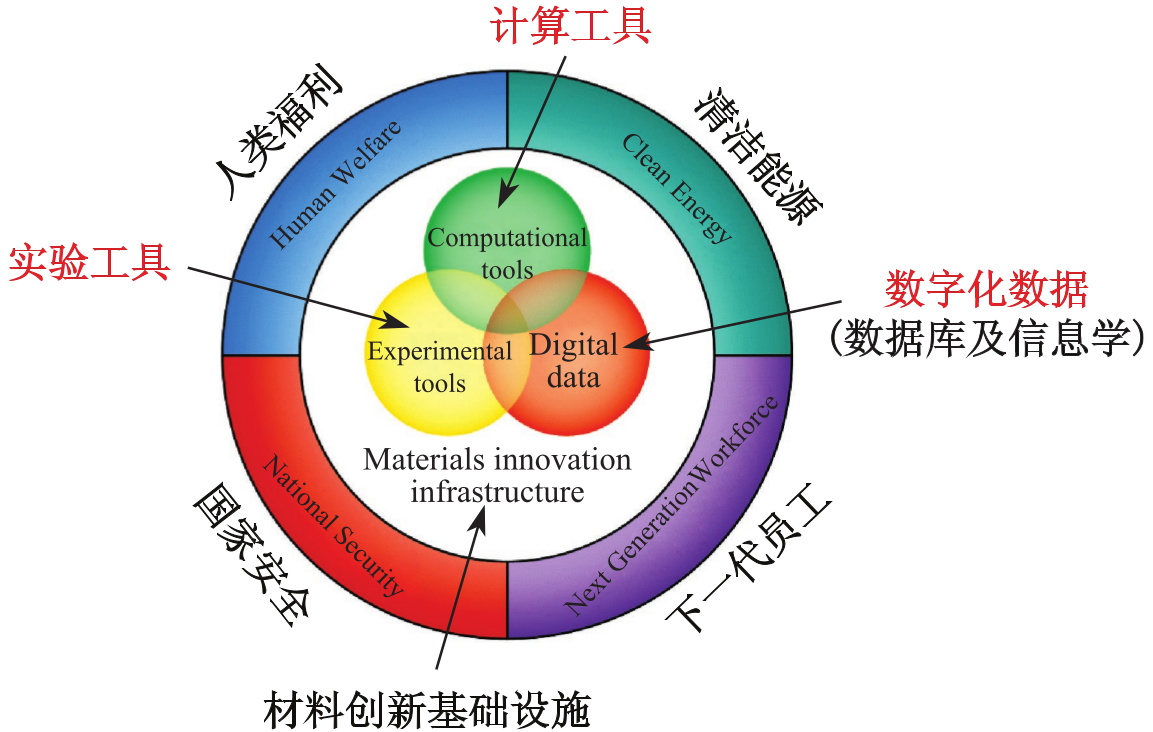
\includegraphics[width=0.6\textwidth]{Figures/Mat_Geno_Ene-1.png}
\vskip 0.10in
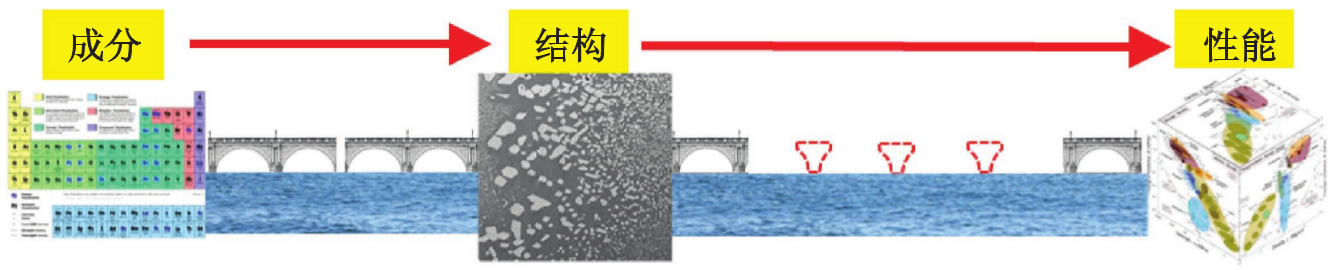
\includegraphics[height=0.85in]{Figures/Mat_Geno_Ene-3.png}
\label{Mater_Genome}
\end{figure}
}

\frame
{
\begin{figure}[h!]
\vskip -5pt
\centering
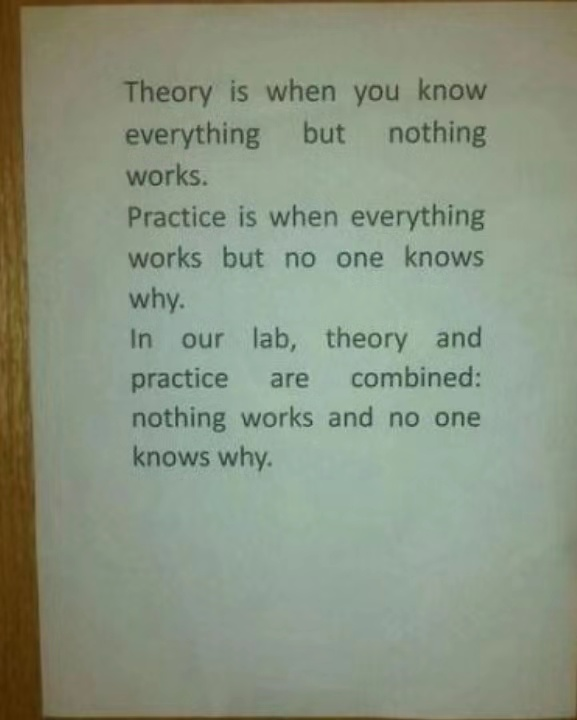
\includegraphics[height=2.8in,width=2.5in,viewport=110 225 505 660,clip]{Figures/Theory_Practice.jpg}
\label{Theory_Practice}
\end{figure}
}

\frame
{
	\frametitle{材料物性模拟的基本思想}
\begin{figure}[h!]
\vspace*{-0.25in}
\centering
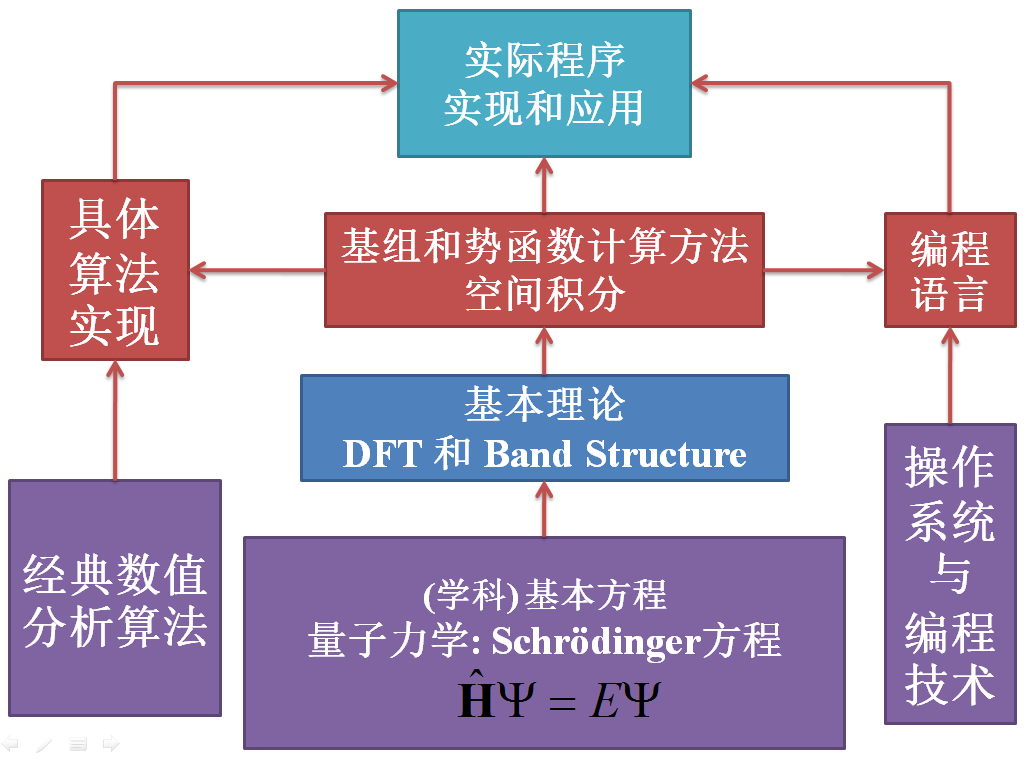
\includegraphics[height=2.80in,width=4.95in,viewport=5 3 1250 780,clip]{Figures/Method_Procedure.png}
%\caption{\small \textrm{Pseudopotential for metallic sodium, based on the empty core model and screened by the Thomas-Fermi dielectric function.}}%(与文献\cite{EPJB33-47_2003}图1对比)
\label{Method-Procedure}
\end{figure}
}

\frame
{
	\frametitle{第一原理尺度计算框架:~\textrm{DFT-SCF}}
\begin{figure}[h!]
\centering
\vspace*{-0.25in}
\hspace*{-0.80in}
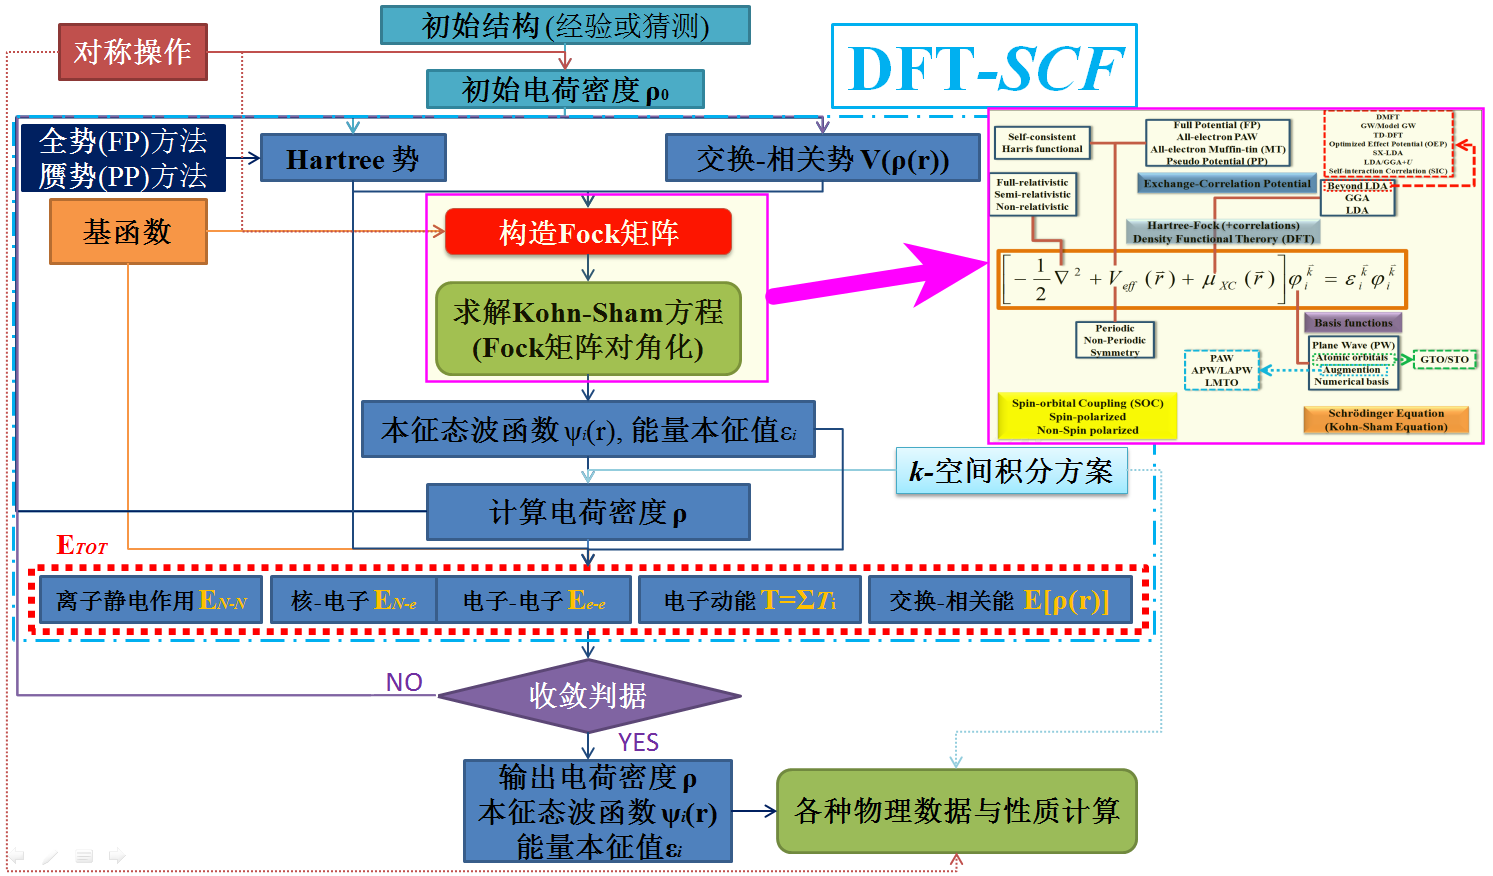
\includegraphics[height=2.80in,width=4.95in,viewport=5 3 1490 870,clip]{Figures/DFT-SCF_2.png}
%\caption{\small \textrm{Pseudopotential for metallic sodium, based on the empty core model and screened by the Thomas-Fermi dielectric function.}}%(与文献\cite{EPJB33-47_2003}图1对比)
\label{Pseudo-NC}
\end{figure}
}

\subsection{材料计算平台开发现状}     %Bookmark
\frame
{
	\frametitle{国内已有的计算平台:~\textrm{MatCloud}}
\begin{figure}[h!]:
\centering
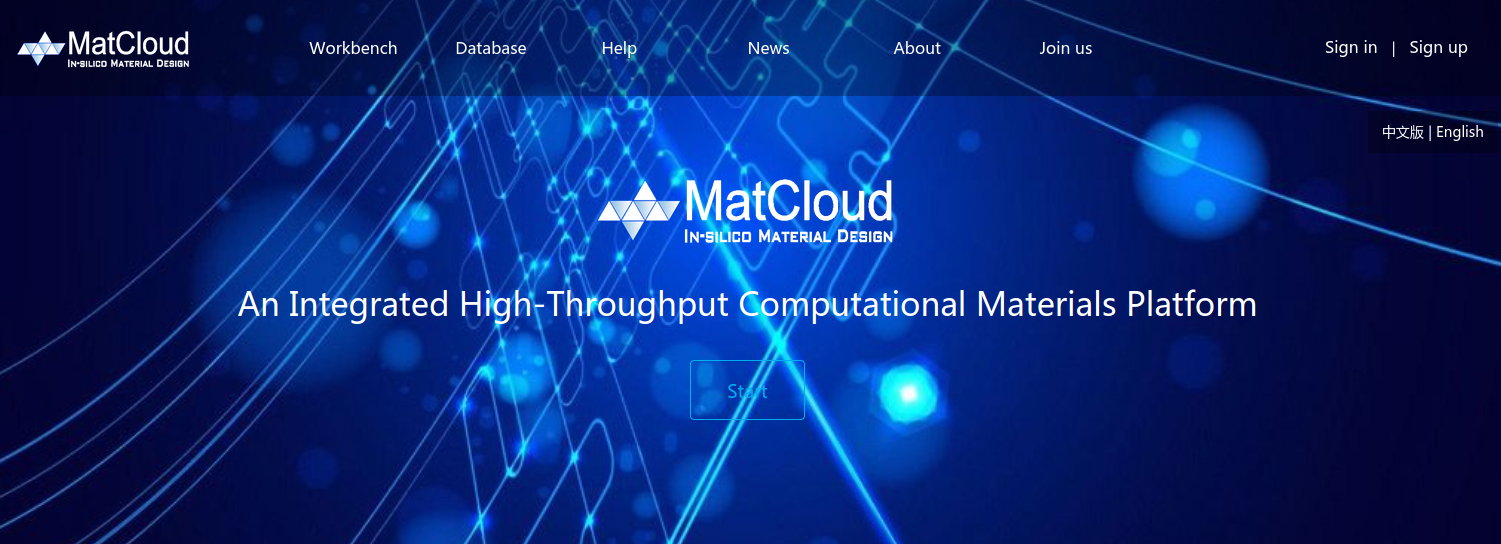
\includegraphics[height=1.57in,width=4.95in,viewport=0 0 1800 550,clip]{Figures/Matcloud-login.png}
\caption{\fontsize{7.2pt}{4.2pt}\selectfont{中科院计算机网络信息中心~杨小渝研究员~团队~开发}\upcite{CMS146-319_2018,url_Matcloud}}%
\label{Auto_Flow_Platform-2}
\end{figure}
}

\frame
{
	\frametitle{国外已有的计算平台}
\begin{figure}[h!]
\centering
\vspace{-15.5pt}
\subfigure[\fontsize{7.5pt}{6.2pt}\selectfont{\textrm{Auto-FLOW (AFLOW)}\upcite{CMS58-227_2012}}]{
\label{AFLOW_data_flow}
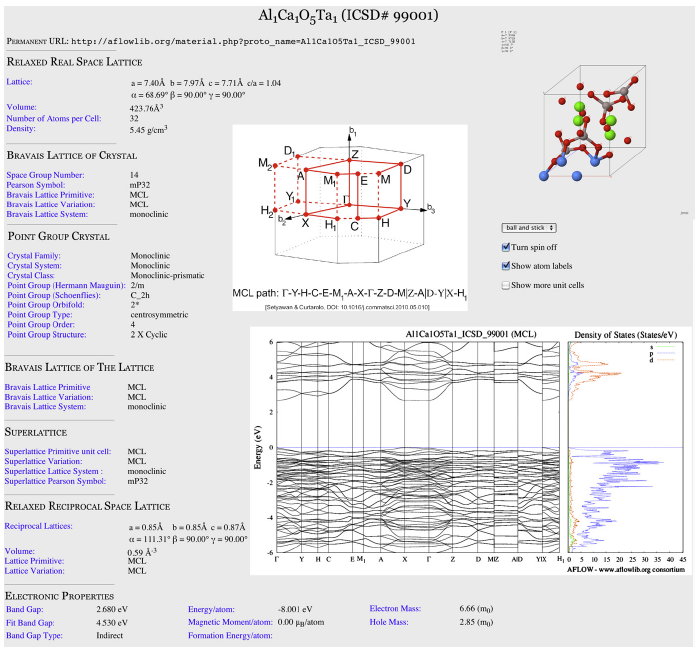
\includegraphics[height=1.2in,width=1.6in,viewport=0 0 720 660,clip]{Figures/AFLOW_database.png}}
\subfigure[\fontsize{7.5pt}{6.2pt}\selectfont{\textrm{Material Project (MP)}\upcite{CMS97-209_2015}}]{
\label{MP_commp_infrastructure}
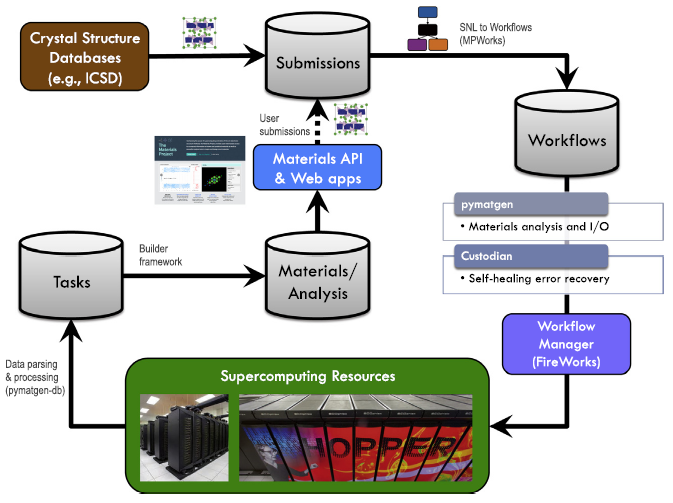
\includegraphics[height=1.2in,width=1.7in,viewport=0 0 670 530,clip]{Figures/MP_comp_infrastructure.png}}
\subfigure[\fontsize{3.5pt}{3.2pt}\selectfont{\textrm{Quantum Materials Informatics Project (QMIP)}\upcite{url_QMIP}}]{
\label{QMIP_Shame}
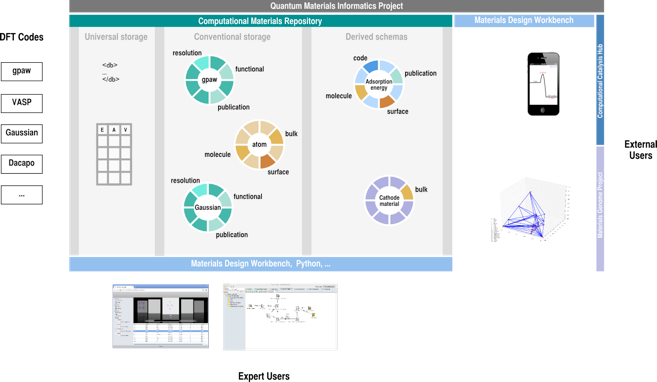
\includegraphics[height=1.2in,width=1.7in,viewport=0 0 670 420,clip]{Figures/QMIP_shame.png}}
\subfigure[\fontsize{6.5pt}{5.2pt}\selectfont{\textrm{Clean Energy Project (CEP)}\upcite{JPCL2-2241_2011}}]{
\label{CEP_structure_flow}
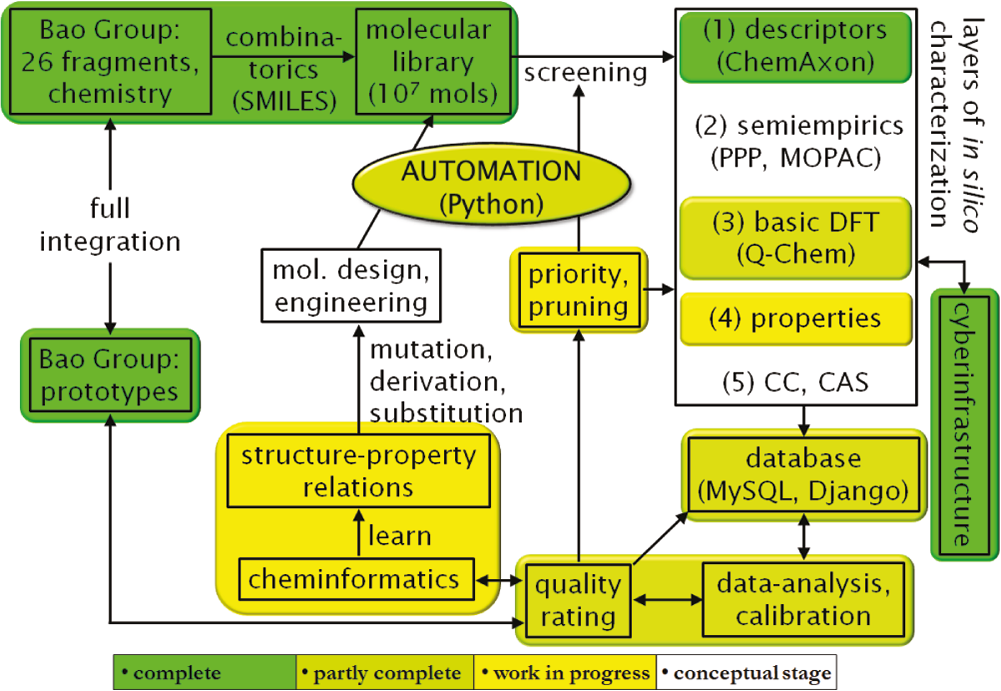
\includegraphics[height=1.2in,width=1.6in,viewport=0 0 1020 730,clip]{Figures/CEP_structure_flow.png}}
%\caption{}%
\label{Auto_Flow_Platform-1}
\end{figure}
}

\frame
{
	\frametitle{\textrm{ASE}:~接口丰富的适应性计算平台}
\begin{figure}[h!]
\centering
\vspace*{-0.2in}
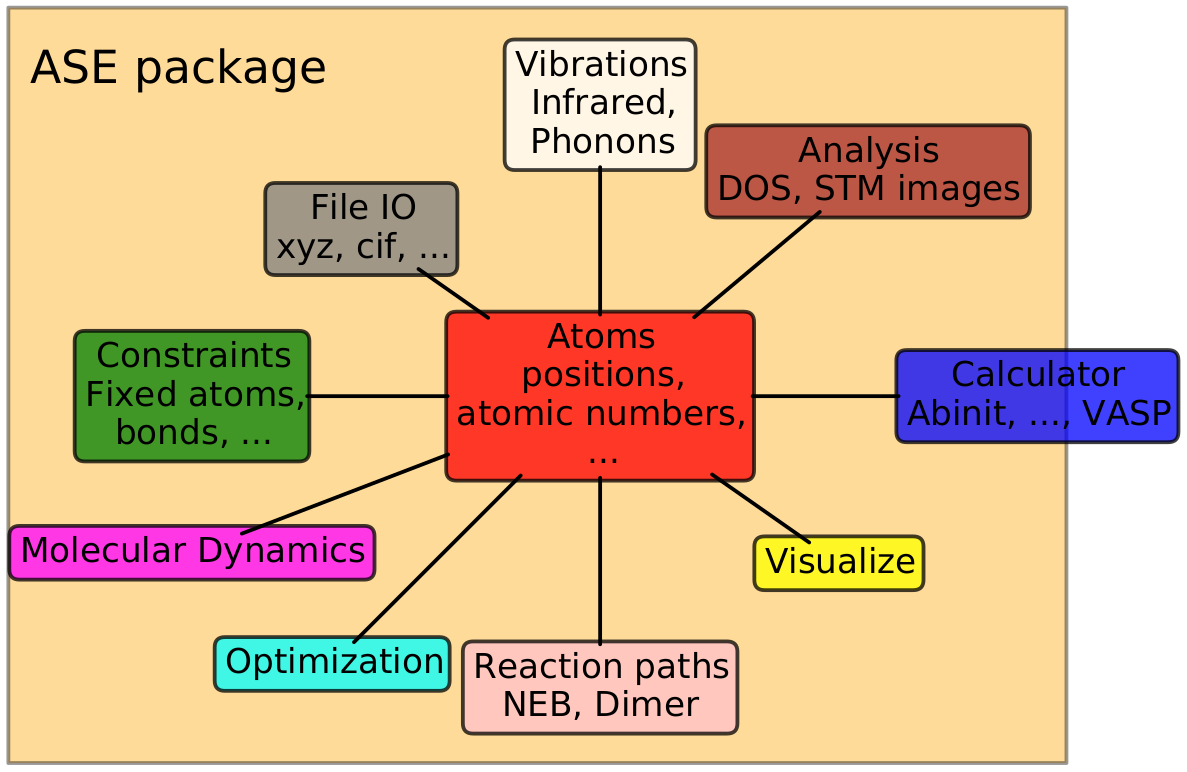
\includegraphics[height=2.1in,width=3.2in,viewport=0 0 1208 830,clip]{Figures/ASE_Python_lib.png}
\caption{\fontsize{7.2pt}{4.2pt}\selectfont{\textrm{ASE:~a Python library for working with atoms.}}}%
\label{Logo_ASE_lib}
\end{figure} 
}

\frame
{
	\frametitle{现有高通量计算平台概览}
\begin{table}[!h]
\tabcolsep 0pt \vspace*{-12pt}
%\caption{}
\label{Table-Cost}
\begin{minipage}{0.85\textwidth}
%\begin{center}
\centering
\def\temptablewidth{1.1\textwidth}
\renewcommand\arraystretch{0.8} %表格宽度控制(普通表格宽度的两倍)
\rule{\temptablewidth}{1pt}
\begin{tabular*} {\temptablewidth}{@{\extracolsep{\fill}}c@{\extracolsep{\fill}}c@{\extracolsep{\fill}}c@{\extracolsep{\fill}}c@{\extracolsep{\fill}}c@{\extracolsep{\fill}}c@{\extracolsep{\fill}}c}
%-------------------------------------------------------------------------------------------------------------------------
	&\multirow{2}{*}{\fontsize{7.2pt}{5.2pt}\selectfont{编程语言}}	&\fontsize{7.2pt}{5.2pt}\selectfont{建模} &\multicolumn{2}{|c|}{\fontsize{6.2pt}{5.2pt}\selectfont{任务提交与管理}} &\multirow{2}{*}{\fontsize{7.2pt}{5.2pt}\selectfont{后处理}} &\multirow{2}{*}{\fontsize{6.2pt}{5.2pt}\selectfont{数据组织管理}} \\\cline{4-5}
	&	&\fontsize{7.2pt}{5.2pt}\selectfont{功能} &\multicolumn{1}{|l}{\fontsize{7.2pt}{5.2pt}\selectfont{软件接口}} &\multicolumn{1}{r|}{\fontsize{7.2pt}{5.2pt}\selectfont{运行容错}} & & \\\hline
	\fontsize{7.2pt}{5.2pt}\selectfont{{AFLOW}} &\fontsize{7.2pt}{5.2pt}\selectfont{C++} &\checkmark &\triangle &\FiveStarOpen &\FiveStarOpen &\fontsize{7.2pt}{5.2pt}\selectfont{{Django}} \\
	\fontsize{7.2pt}{5.2pt}\selectfont{{MP}} &\fontsize{7.2pt}{5.2pt}\selectfont{Python} &\checkmark &\checkmark &\FiveStarOpen &\FiveStarOpen &\fontsize{7.2pt}{5.2pt}\selectfont{{MongoDB}} \\
	\multirow{2}{*}{\fontsize{7.2pt}{5.2pt}\selectfont{{QMIP}}} &\fontsize{7.2pt}{5.2pt}\selectfont{JavaScript/SVG} &\multirow{2}{*}{\checkmark} &\multirow{2}{*}{\checkmark} &\multirow{2}{*}{--} &\multirow{2}{*}{\checkmark} &\multirow{2}{*}{--} \\
	&\fontsize{7.2pt}{5.2pt}\selectfont{+html/Python} & & & & & \\
	\fontsize{7.2pt}{5.2pt}\selectfont{{CEP}} &\fontsize{7.2pt}{5.2pt}\selectfont{Python} &\checkmark &\checkmark &-- &\checkmark &\fontsize{7.2pt}{5.2pt}\selectfont{{Django/MySQL}} \\
	\fontsize{7.2pt}{5.2pt}\selectfont{{ASE}} &\fontsize{7.2pt}{5.2pt}\selectfont{Python} &\FiveStarOpen &\FiveStarOpen &-- &\triangle &-- \\
	\multirow{2}{*}{\fontsize{7.2pt}{5.2pt}\selectfont{{MatCloud}}} &\fontsize{7.2pt}{5.2pt}\selectfont{JavaScript} &\multirow{2}{*}{\checkmark} &\multirow{2}{*}{\triangle} &\multirow{2}{*}{\checkmark} &\multirow{2}{*}{\checkmark} &\multirow{2}{*}{\fontsize{7.2pt}{5.2pt}\selectfont{{MongoDB}}} \\
	&\fontsize{7.2pt}{5.2pt}\selectfont{+.NETCore} & & & & &
\end{tabular*}
\rule{\temptablewidth}{1pt}
\end{minipage}
%\vskip -15pt
\fontsize{7.2pt}{5.2pt}\selectfont{
\begin{description}
	\item[\FiveStarOpen]~该功能较突出
	\item[\checkmark]~该功能基本满足需求
	\item[\triangle]~该功能存在不足
\end{description}}
%\end{center}
\end{table}
}

\frame
{
	\frametitle{\textrm{软件开发:~理想与现实}}
\begin{figure}[h!]
\centering
\vspace*{-0.26in}
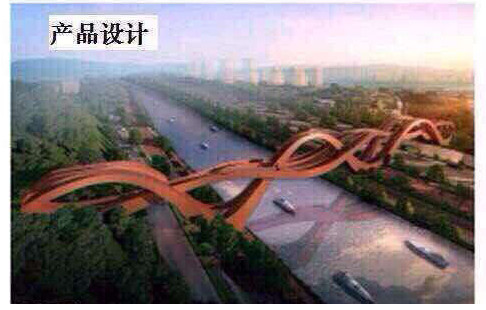
\includegraphics[height=0.9in,width=1.5in,viewport=0 0 120 80,clip]{Figures/Product_plan_tech_02.jpg}
\vskip 1pt
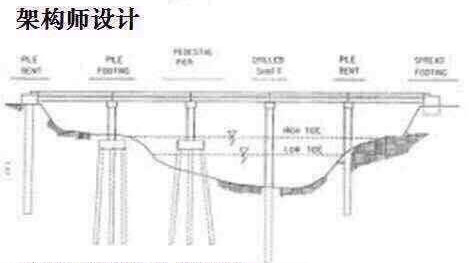
\includegraphics[height=0.8in,width=1.5in,viewport=0 0 120 70,clip]{Figures/Product_plan_tech_03.jpg}
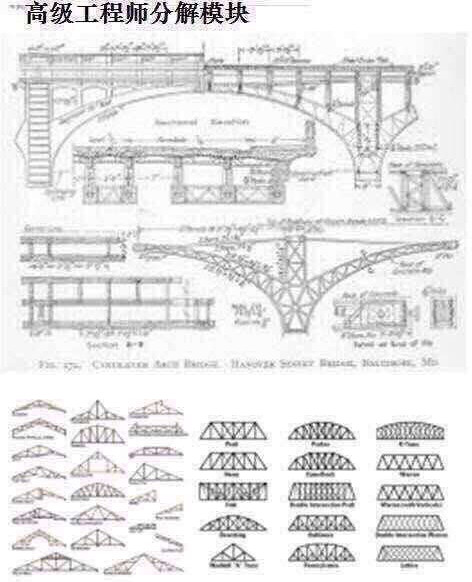
\includegraphics[height=1.2in,width=1.0in,viewport=0 0 120 140,clip]{Figures/Product_plan_tech_04.jpg}
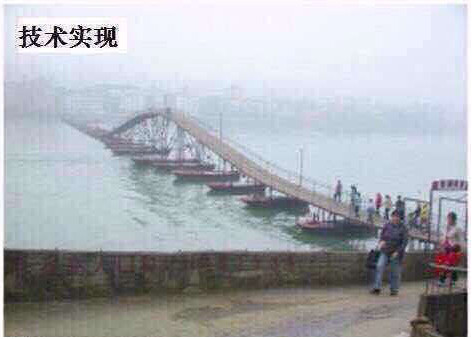
\includegraphics[height=0.9in,width=1.5in,viewport=0 0 120 80,clip]{Figures/Product_plan_tech_06.jpg}
\vskip 1pt
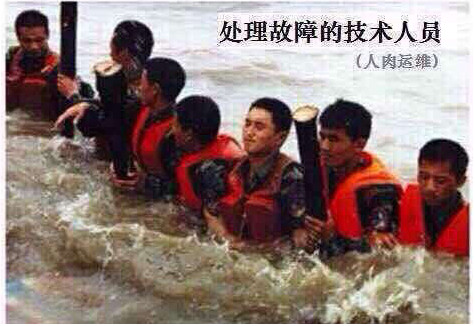
\includegraphics[height=0.9in,width=1.5in,viewport=0 0 120 80,clip]{Figures/Product_plan_tech_08.jpg}
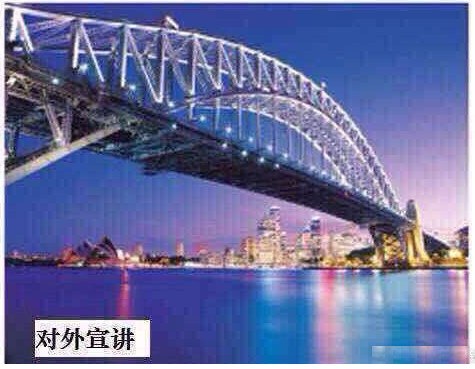
\includegraphics[height=0.9in,width=1.5in,viewport=0 0 120 80,clip]{Figures/Product_plan_tech_09.jpg}
%\caption{\fontsize{7.2pt}{4.2pt}\selectfont{\textrm{The integrated calculator in ASE (Atomic Simulation Environment).}}}%
\label{Product_plan_tech}
\end{figure} 
}

\subsection{异质界面催化模拟自动流程软件设计与开发}
\frame
{
	\frametitle{\textrm{一般材料计算平台的功能和总体架构}}
\begin{figure}[h!]
\centering
\hspace*{-0.2in}
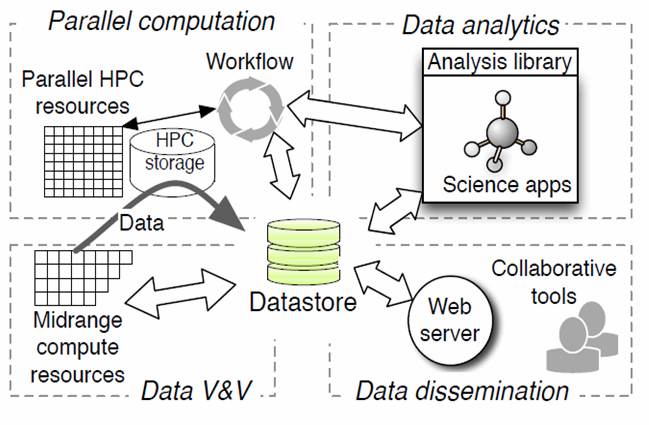
\includegraphics[height=1.25in,width=1.95in,viewport=0 0 670 460,clip]{Figures/Parallel_computation.png}
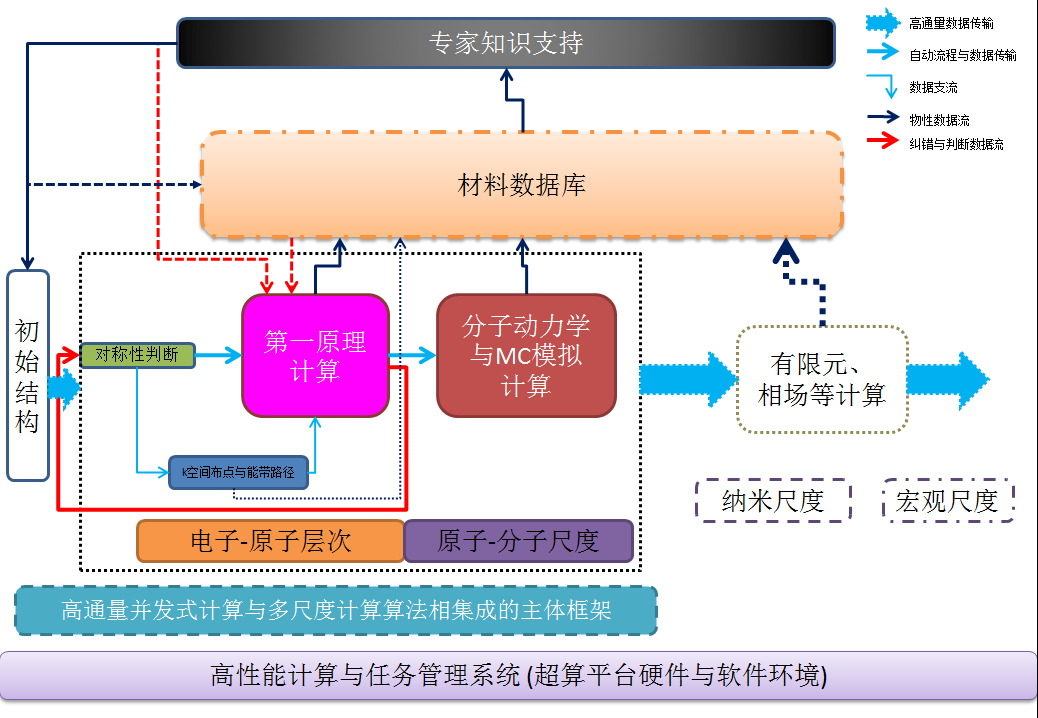
\includegraphics[height=1.6in,width=2.4in,viewport=0 0 1038 730,clip]{Figures/Auto_Flow.png}
\caption{\fontsize{7.2pt}{4.2pt}\selectfont{\textrm{The schematic framework and platform of all those project.}}}%
\label{Auto_Flow}
\end{figure} 
}

\frame
{
	\frametitle{适应异质界面催化模拟自动流程软件开发}
\begin{minipage}[b]{0.47\linewidth}
	\begin{itemize}
		\item \fontsize{8.0pt}{4.2pt}\selectfont{适用于异质界面的高通量材料计算自动流程软件架构}
\begin{figure}[h!]
\centering
\hskip -35pt
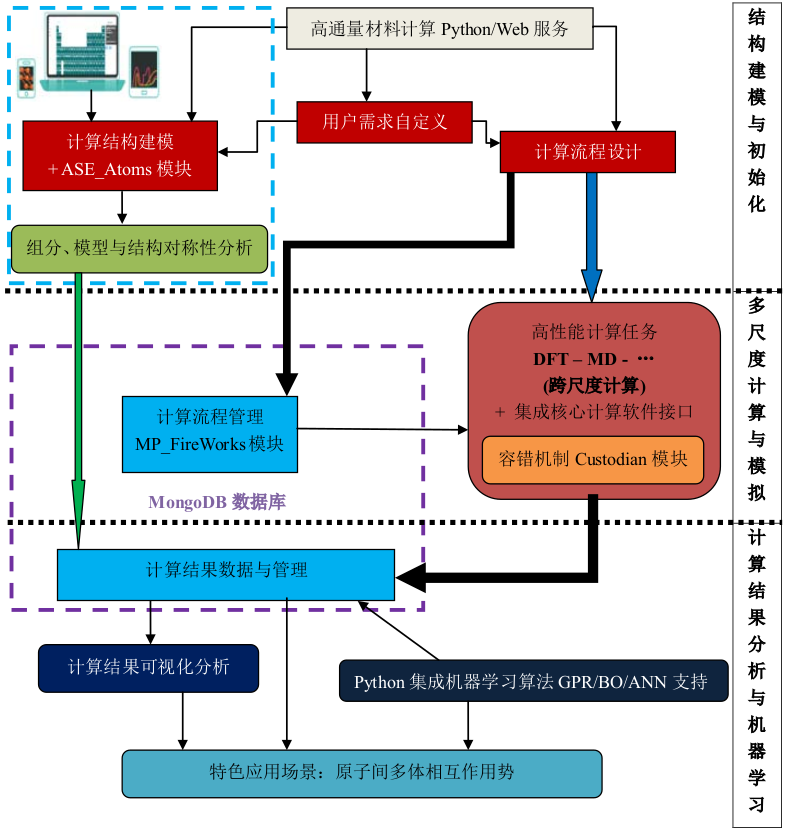
\includegraphics[height=2.18in]{Figures/MP_comp_BCC.png}
%\caption{\fontsize{6.5pt}{4.2pt}\selectfont{适应多体相互作用的高通量计算流程结构示意}}%
\label{MP_comp_BCC}
\end{figure}
	\end{itemize}
\end{minipage}
~
\begin{minipage}[b]{0.42\linewidth}
\begin{itemize}
%	\item “标准化”对称性分析功能:~降低\textrm{DFT}的计算量
	\item \textcolor{magenta}{高性能计算集群}:~提升电子计算的规模%,为\textrm{DFT-MD}计算提供基础
	\item \textcolor{magenta}{机器学习}:~优化电子计算结果,获得\textrm{MD}尺度力场,\textrm{DFT-MD}耦合%,获得\textrm{MD}尺度下准确的多体相互作用的力场函数。
	\item 设计合理完善的程序流程:~利用\textrm{MongoDB}支持的\textrm{FireWorks}计算流程管理%,由微观尺度\textrm{DFT}计算获得介观或宏观尺度的计算物性或者使不同尺度的计算结果更好地实现耦合自洽
\end{itemize}
\end{minipage}
}

\frame
{
	\frametitle{\rm{DFT-MD}耦合:~催化反应机理模拟流程}
\begin{enumerate}
	\item \fontsize{8.7pt}{6.2pt}\selectfont{\textrm{FireWorks}流程框架支持初始\textrm{DFT}计算并发}
	%\item 为\textrm{DFT}尺度下的原子间相互作用,启动并发式\textrm{Kohn-Sham}方程求解和化学反应动力学(反应通道)计算
	\item \fontsize{8.7pt}{6.2pt}\selectfont{筛选活化能最小的反应通道}%(\textrm{DFT-MD}尺度筛选)
%	\item \textrm{DFT}尺度下,多种结构的反应活化能计算,根据活化能确定可能的决速步
	\item \fontsize{8.7pt}{6.2pt}\selectfont{优化决速步原子间相互作用函数}%(\textrm{DFT-MD}跨尺度耦合)
	\item \fontsize{8.7pt}{6.2pt}\selectfont{求解原子的\textrm{MD}运动方程}
	\item \fontsize{8.7pt}{6.2pt}\selectfont{经\textrm{MD}模拟后确定当前体系各原子结构,返回决速步,\textrm{DFT}再次计算活化能}
	\item \fontsize{8.7pt}{6.2pt}\selectfont{迭代循环,筛选出可能的决速步,得到稳定的催化燃烧反应动力学流程,直至收敛}
\end{enumerate}
\begin{figure}[h!]
\centering
\vskip -2pt
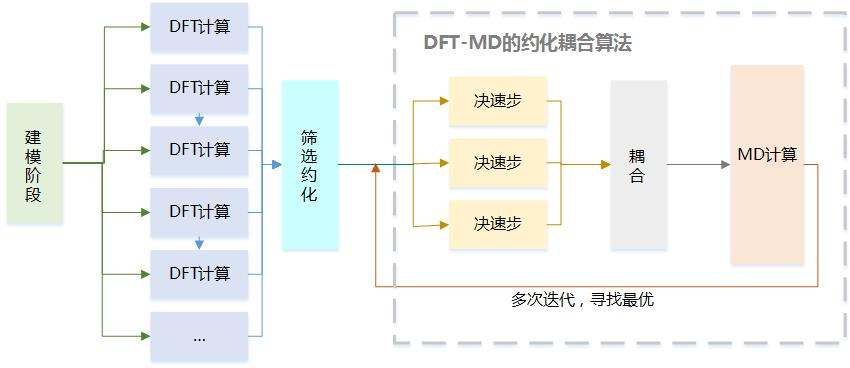
\includegraphics[height=1.05in]{Figures/CH4_complex_machine.png}
\hskip 1pt
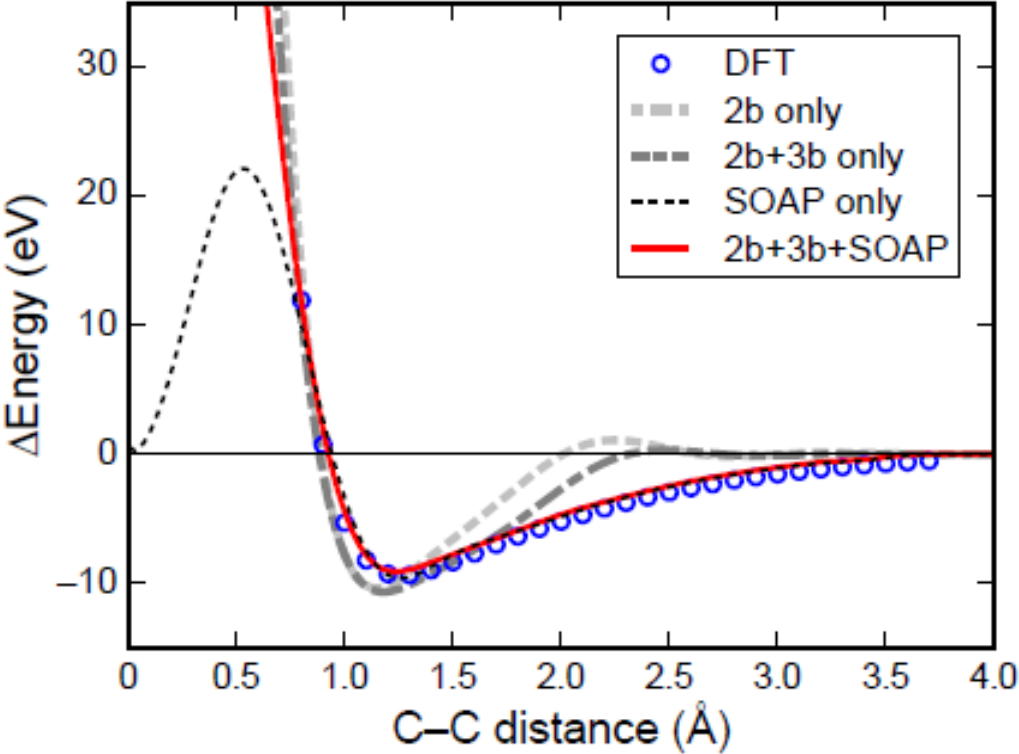
\includegraphics[height=1.05in]{Figures/poten-TiO2.png}%}
\caption{\fontsize{5.5pt}{4.2pt}\selectfont{面向催化燃烧反应动力学机理模拟的计算自动流程示意图}}%
\label{CH4_comp_BCC}
\end{figure}
}

\subsection{实现与技术:~\rm{MP}与\rm{ASE}}     %Bookmark
\frame
{
	\frametitle{\textrm{MP}自动流程的设计与开发}
	\begin{itemize}
		\item \textcolor{red}{设计目标}:~围绕\textrm{VASP~}作业高通量并发提交与过程监控
		\item \textcolor{red}{设计方案}:~开发针对不同计算场景的功能模块
			\begin{enumerate}
    \setlength{\itemsep}{15pt}
				\item \textcolor{blue}{\textbf{Pymatgen}}\\
					\textcolor{magenta}{前处理}:~计算模型的分析与预处理\\
					\textcolor{magenta}{后处理}:~计算结果的可视化
				\item \textcolor{blue}{\textbf{FireWorks}}\\
\textcolor{magenta}{计算流程设计与管理}:~数据库支持的计算流程管理
				\item \textcolor{blue}{\textbf{Custodian}}\\
\textcolor{magenta}{计算流程容错与应对}:~提供计算过程错误判断接口,由用户提供解决策略和针对性设计
			\end{enumerate}
	\end{itemize}
		%\item 计算过程的控制方式
}

\frame
{
	\frametitle{\textrm{Pymatgen}的模块结构}
\begin{figure}[h!]
\centering
\vspace*{-0.1in}
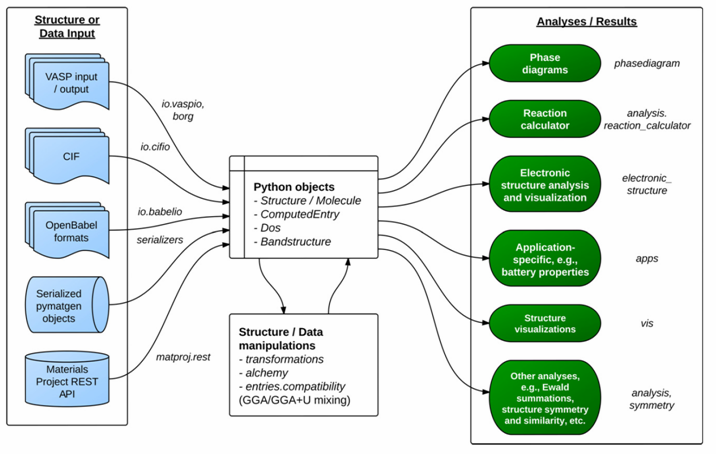
\includegraphics[height=2.3in]{Figures/MP_library.png}
\caption{\fontsize{7.2pt}{4.2pt}\selectfont{\textrm{Overview of a typical workflow for pymatgen.}}}%
\label{Pymatgen_Lib}
\end{figure} 
}

%\frame
%{
%	\frametitle{\textrm{Pymatgen}可展示的材料物性}
%\begin{figure}[h!]
%\centering
%\vspace*{-0.1in}
%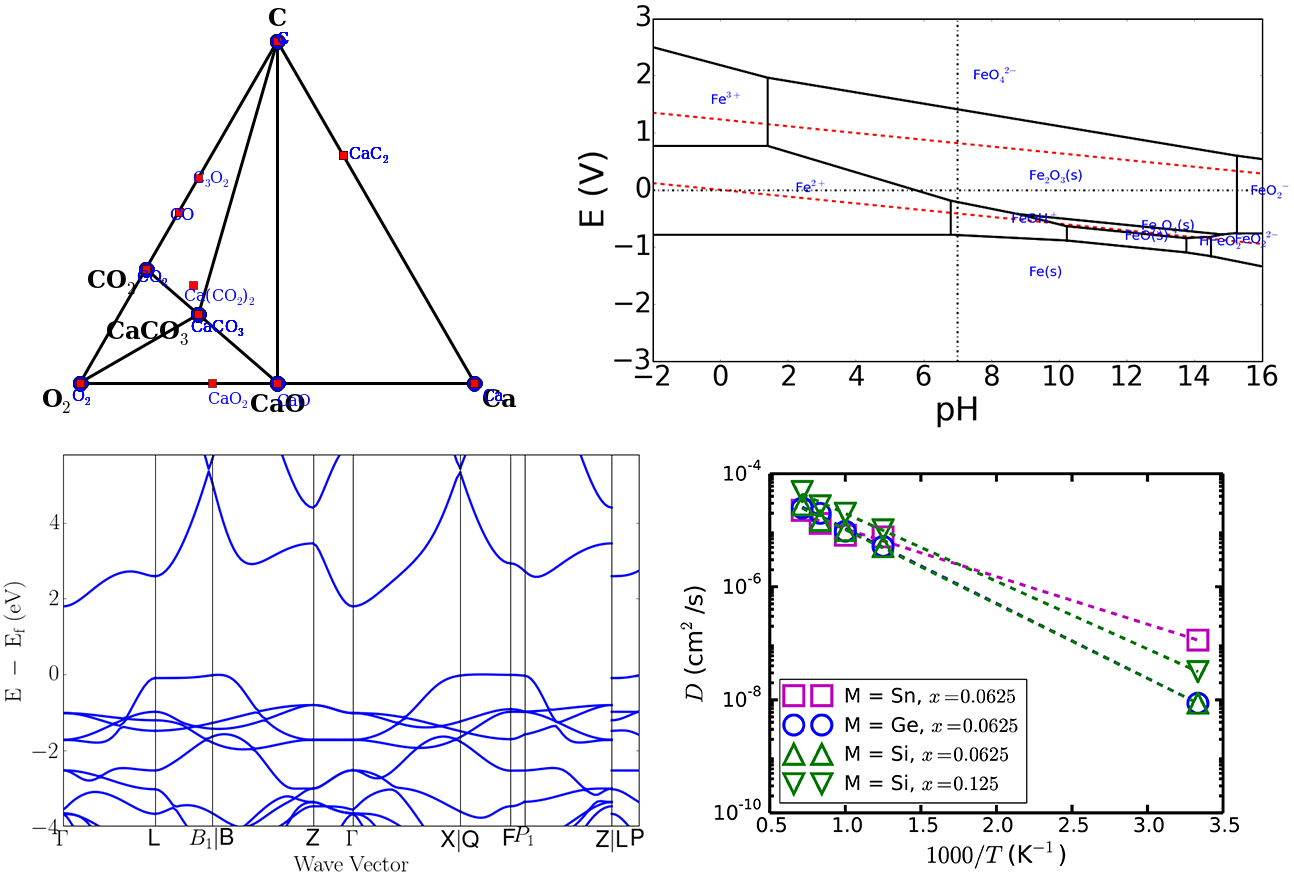
\includegraphics[height=2.3in]{Figures/MP_vision.png}
%\caption{\fontsize{5.2pt}{4.2pt}\selectfont{\textrm{Top left: Phase; Top right: Pourbaix diagram from the Materials API. \\Bottom left: Calculated bandstructure plot using pymatgen’s parsing and plotting utilities. Bottom right: Arrhenius plot using pymatgen’s Diffusion~Analyzer.}}}%
%\label{Pymatgen_vision}
%\end{figure} 
%}
%
\frame
{
	\frametitle{\textrm{FireWorks}的模块结构}
\begin{figure}[h!]
\centering
\vspace*{-0.1in}
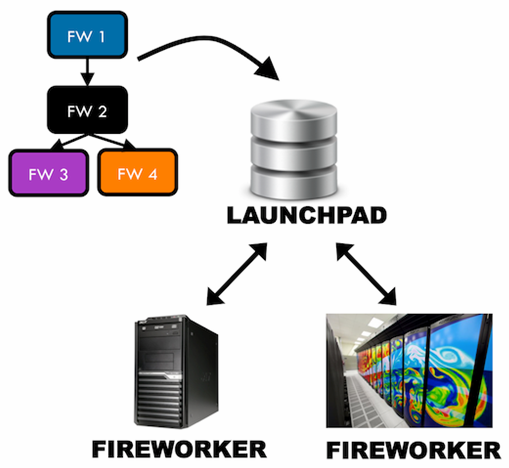
\includegraphics[height=1.6in]{Figures/MP_fireworks.png}
\hskip 1pt
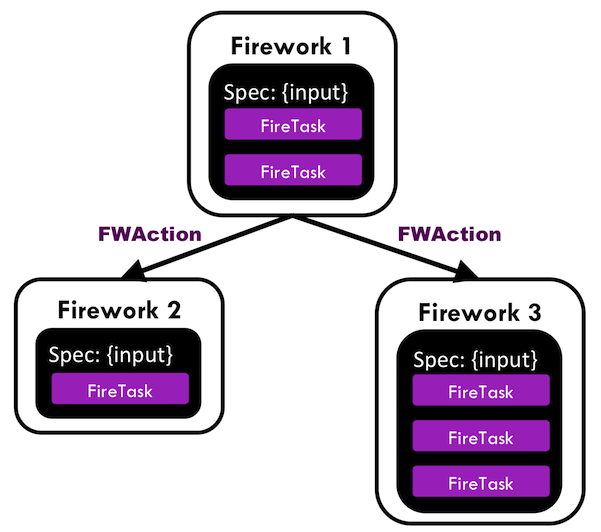
\includegraphics[height=1.6in]{Figures/MP_multiple_fw.png}
\caption{\fontsize{7.2pt}{4.2pt}\selectfont{\textrm{The basic infrastructure of FireWorks.}}}%
\label{FireWorks_FW}
\end{figure} 
\textcolor{magenta}{特色}:~基于数据库支持的计算流程:
\begin{itemize}
	\item 实现了复杂计算流程的模块化与可分离,方便流程的设计、维护和管理
	\item 流程运行过程中少人工干扰
\end{itemize}
}

\frame
{
	\frametitle{\textrm{Custodian}的容错逻辑}
\begin{figure}[h!]
\centering
\vspace*{-0.1in}
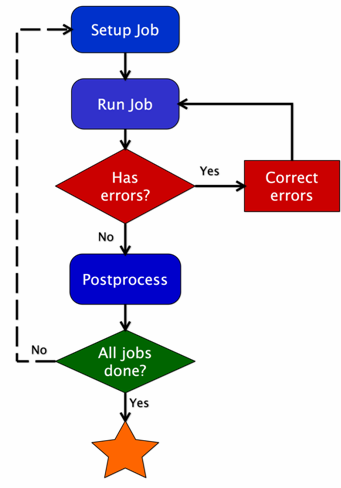
\includegraphics[height=2.3in]{Figures/MP_custodian.png}
\label{Custodian_over}
\caption{\fontsize{7.2pt}{4.2pt}\selectfont{\textrm{Overview of the Custodian workflow.}}}%
\end{figure} 
}

\frame
{
	\frametitle{\textrm{atomate}:~计算流程控制示范}
%		\textcolor{purple}{\textrm{Atomate}}:~:~适合一定复杂程度的\textrm{~VASP~}计算
\begin{figure}[h!]
\centering
\vspace*{-0.1in}
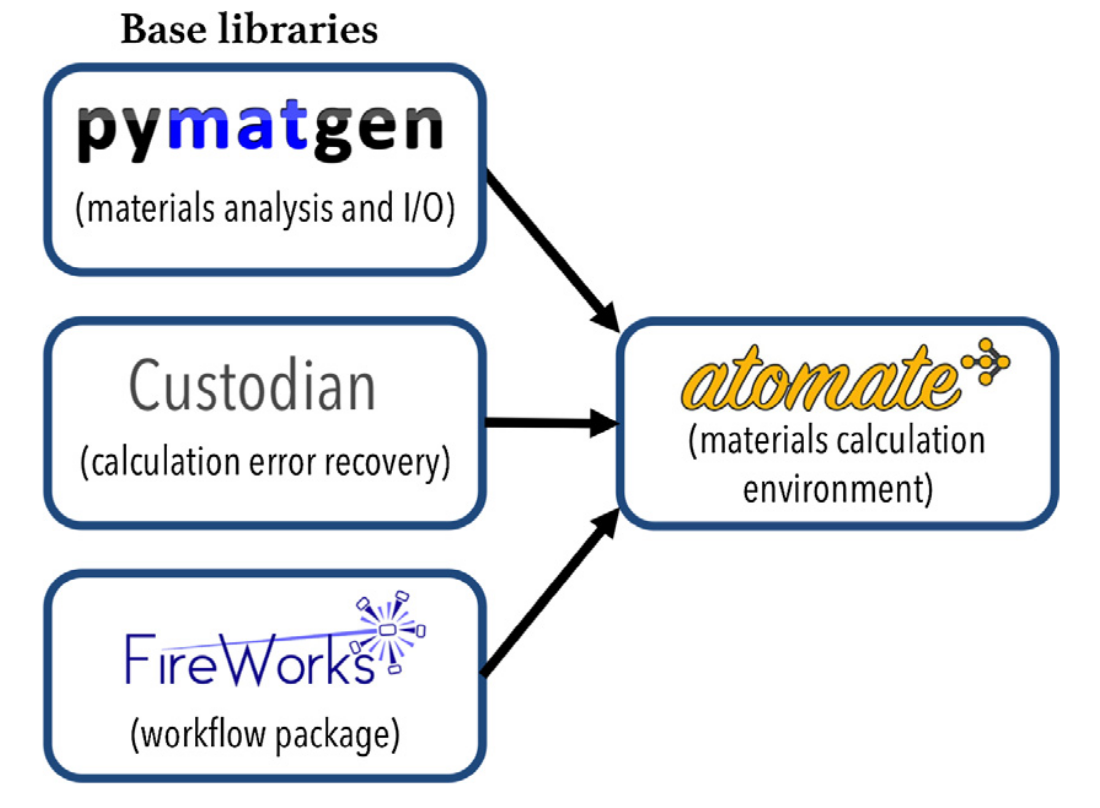
\includegraphics[height=1.3in,width=2.2in,viewport=0 0 820 630,clip]{Figures/Atomate_comp.png}
\vskip 1pt
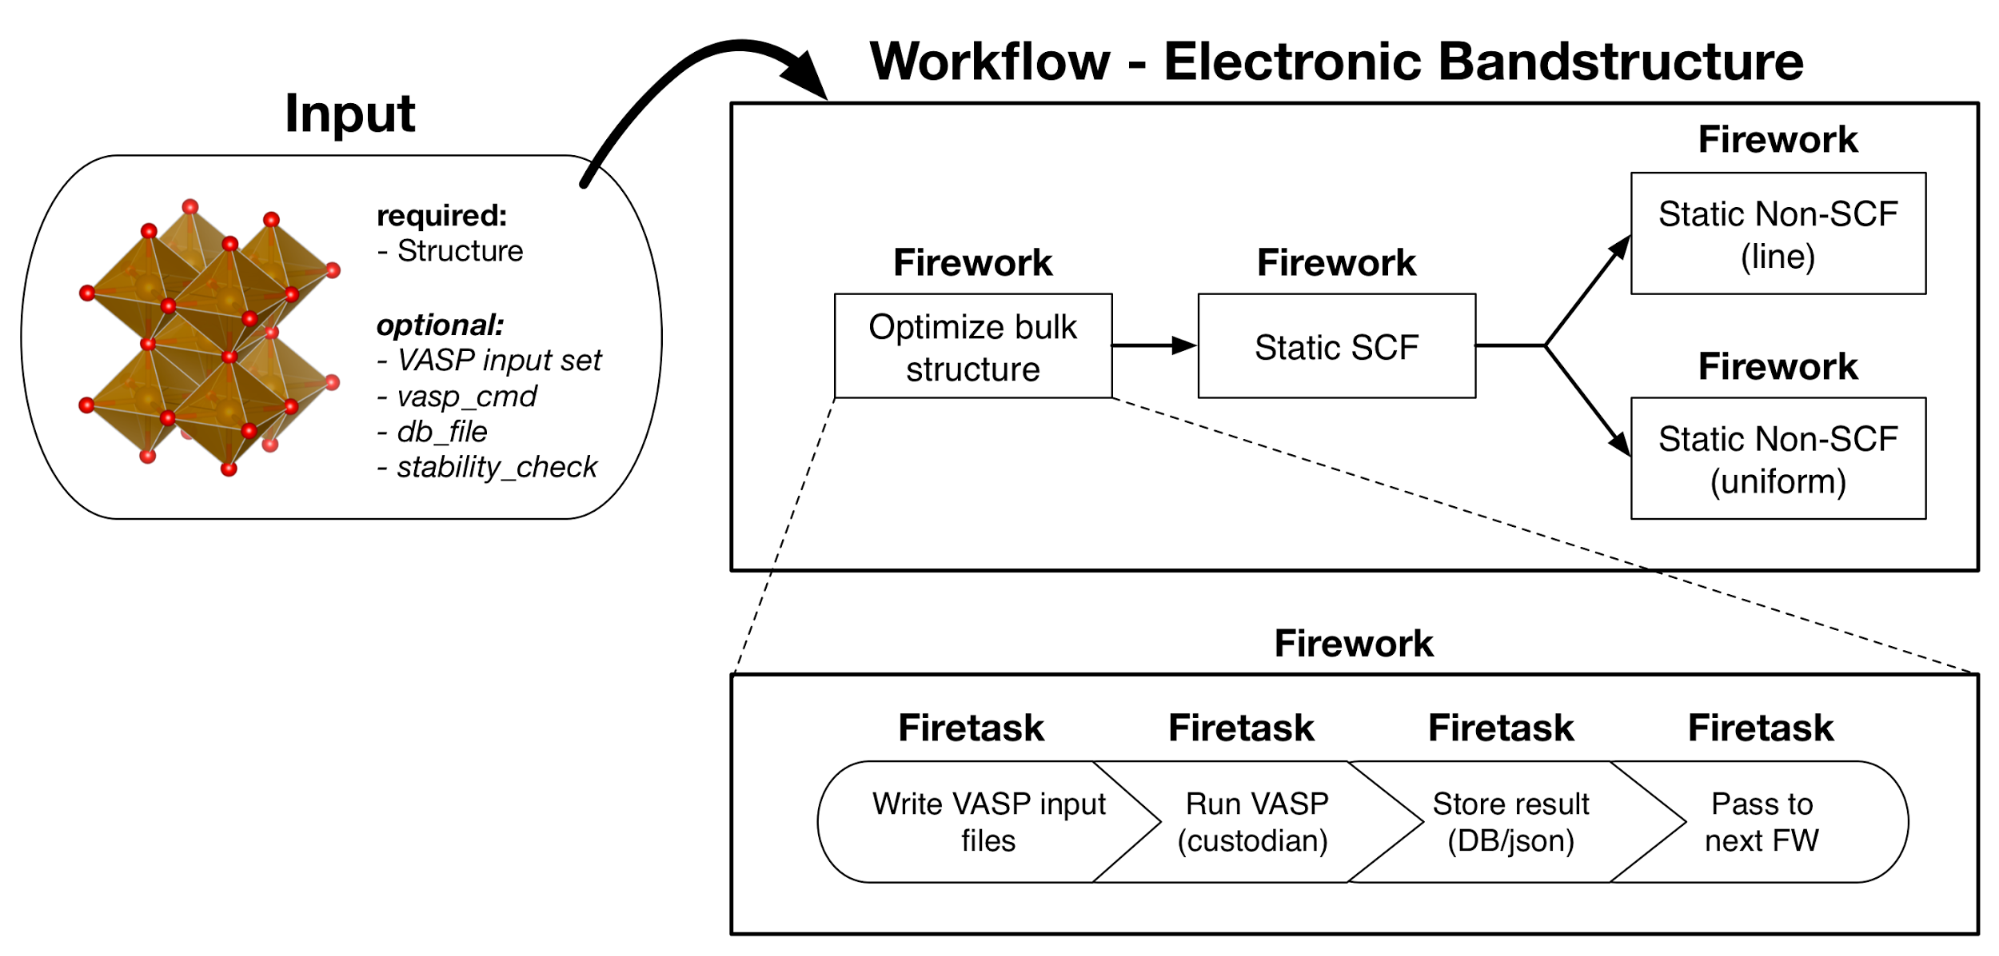
\includegraphics[height=1.5in]{Figures/bandstructure_wf.png}
%\caption{\fontsize{7.2pt}{4.2pt}\selectfont{\textrm{The integrated calculator in ASE (Atomic Simulation Environment).}}}%
\label{Logo_QM-MM}
\end{figure} 
}

\frame
{
	\frametitle{\textrm{ASE}自动流程的设计与管理}
		\textcolor{purple}{\textrm{ASE}}:~模块加载式计算流程控制,更符合复杂多尺度计算场景
		\begin{itemize}
			\item \textcolor{magenta}{灵活的建模功能}
				\begin{enumerate}
    \setlength{\itemsep}{10pt}
					\item 简单堆积:~原子直接组成分子
					\item 理想周期体系(包括一维、二维、三维)
					\item 表面和表面吸附,可指定吸附位
				\end{enumerate}
			\item \textcolor{magenta}{丰富的软件接口}\\
				提供了包括绝大部分第一原理和分子动力学计算软件接口,方便组合实现多尺度计算
			\item \textcolor{magenta}{不依赖软件的优化与动力学模拟}\\
				适合复杂材料物性模拟的优化和多种动力学过程模拟
			\item \textcolor{magenta}{多样化的数据库类型}
		\end{itemize} 
}

\frame
{
\frametitle{\textrm{ASE}特色:~材料结构生成模块}
\begin{figure}[h!]
\centering
\vspace*{-0.27in}
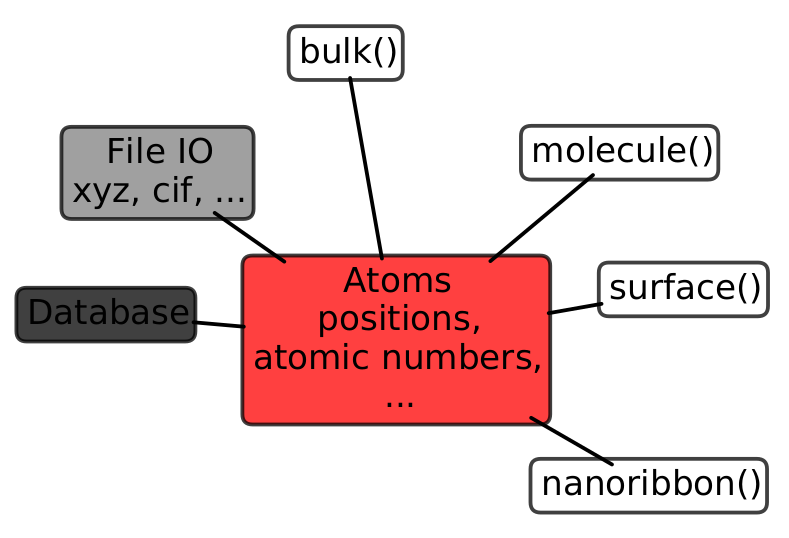
\includegraphics[height=1.3in,width=1.9in,viewport=0 0 820 530,clip]{Figures/ASE_atoms_module.png}
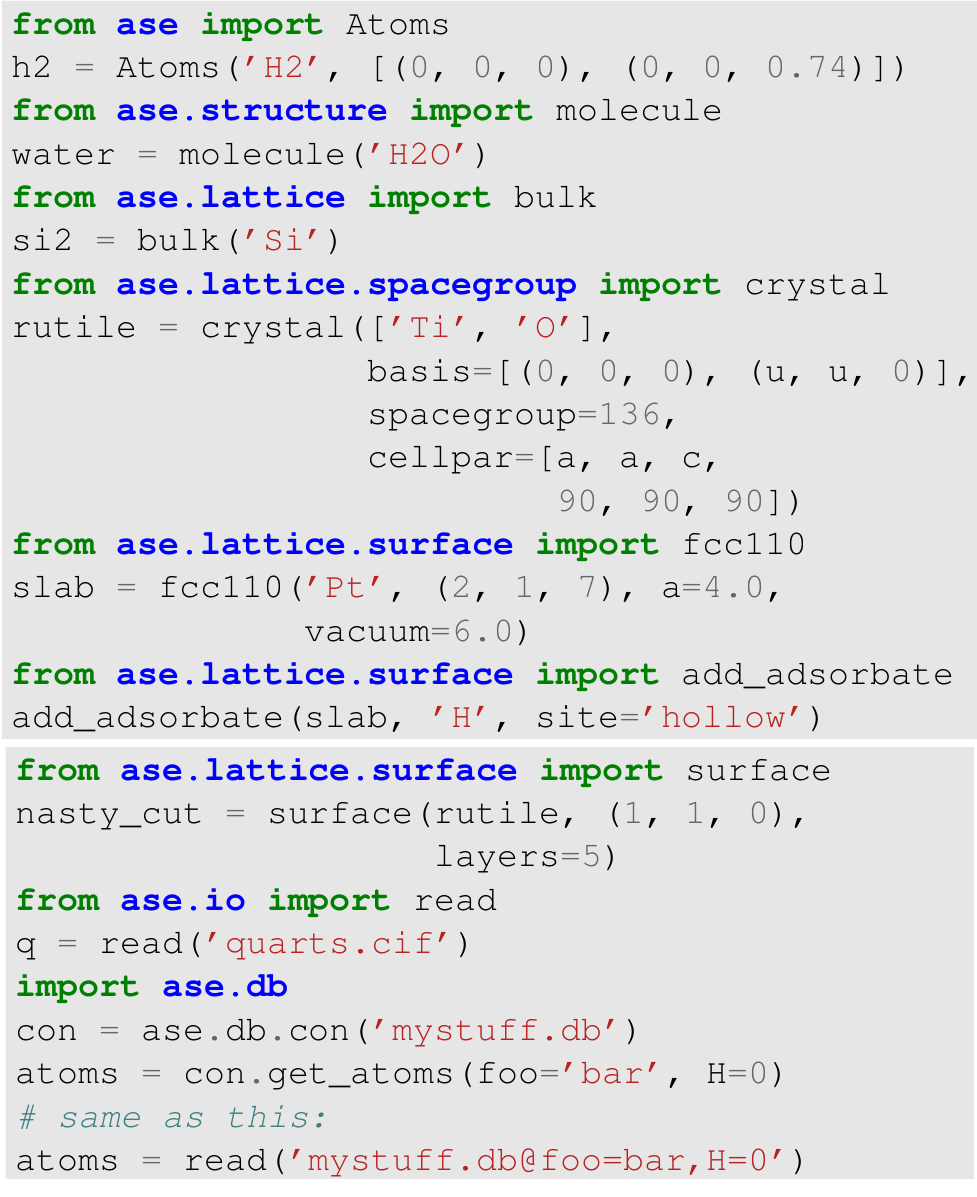
\includegraphics[height=2.9in,width=2.2in,viewport=0 0 970 1200,clip]{Figures/ASE_atoms_module-examples.png}
%\caption{\fontsize{7.2pt}{4.2pt}\selectfont{\textrm{The integrated calculator in ASE (Atomic Simulation Environment).}}}%
\label{Logo_atoms-module}
\end{figure} 
}

\frame
{
\frametitle{\textrm{ASE}特色:~软件接口丰富}
\textcolor{purple}{\textrm{ASE}}:~\textrm{Calculator}模块提供的可选的软件接口
\begin{figure}[h!]
\centering
\vspace*{-0.05in}
%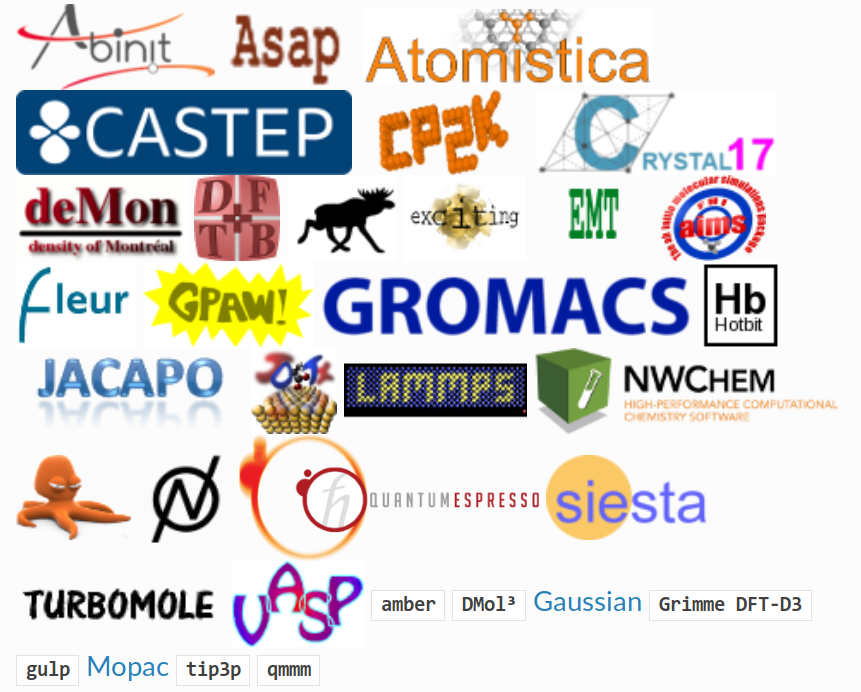
\includegraphics[height=1.0in,width=1.4in,viewport=0 0 638 530,clip]{Figures/ASE_calculator.png}
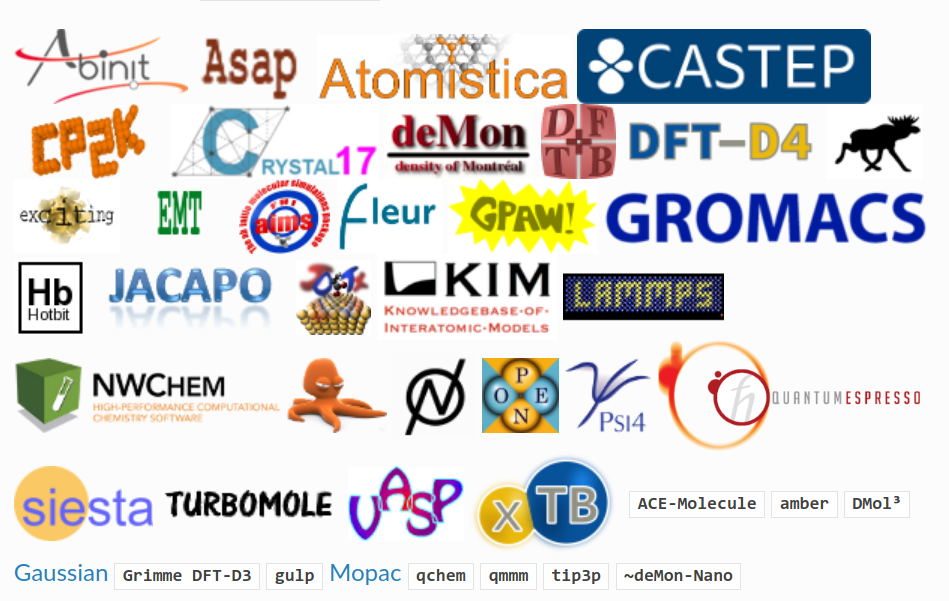
\includegraphics[height=2.0in,width=3.2in,viewport=0 0 940 600,clip]{Figures/ASE_calculator-new.png}
\caption{\fontsize{7.2pt}{4.2pt}\selectfont{\textrm{The integrated calculator in ASE.}}}%
\label{ASE_Calculator}
\end{figure} 
}

\frame
{
\frametitle{\textrm{ASE}特色:~提供多种优化算法模块和数据库}
\begin{figure}[h!]
\centering
\vspace*{-0.21in}
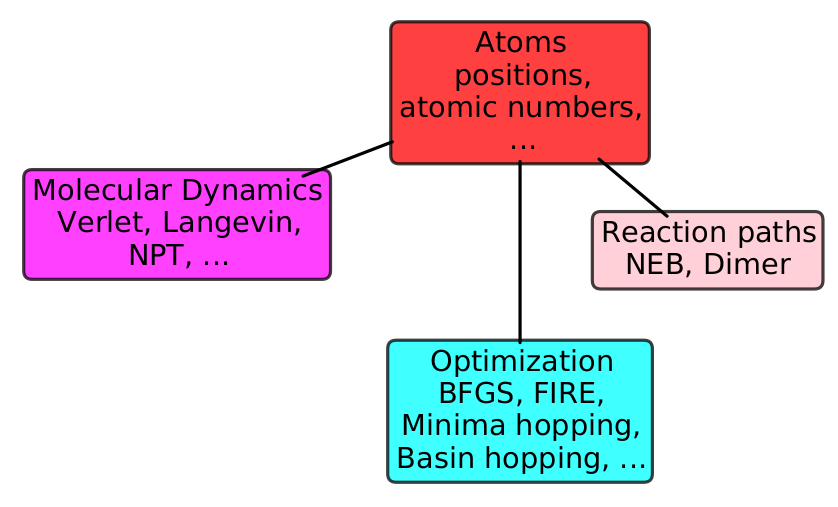
\includegraphics[height=1.3in,width=2.5in,viewport=0 0 838 500,clip]{Figures/ASE_opt_modules.png}
\vskip 1pt
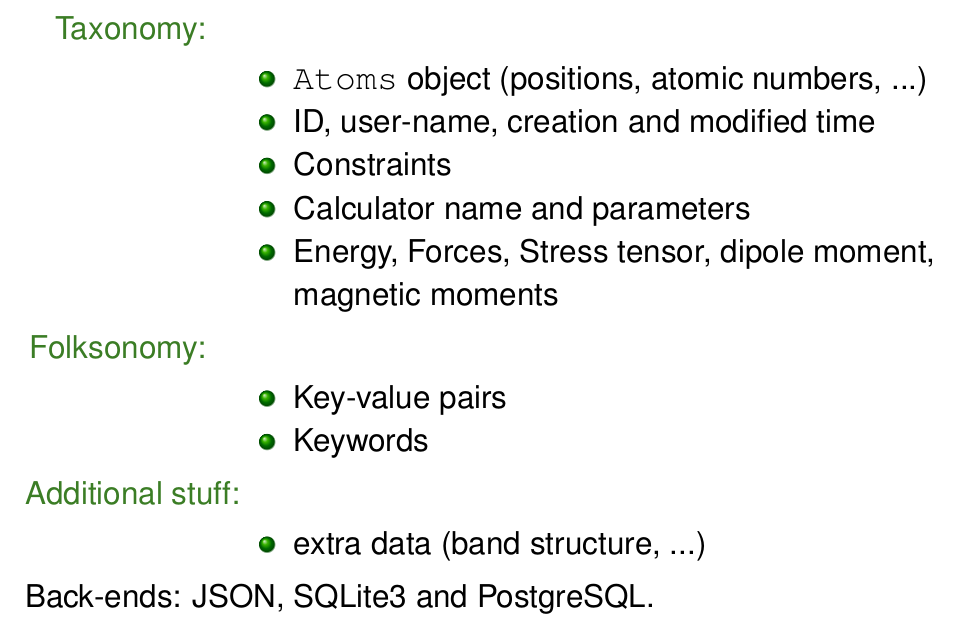
\includegraphics[height=1.7in,width=2.5in,viewport=0 0 938 630,clip]{Figures/ASE_database.png}
\label{ASE_opt-database}
\end{figure} 
}
%\frame
%{
%	\frametitle{\textrm{计算平台的作业自动提交:~基于\textrm{ASE}}}
%\begin{figure}[h!]
%\centering
%\vspace*{-0.2in}
%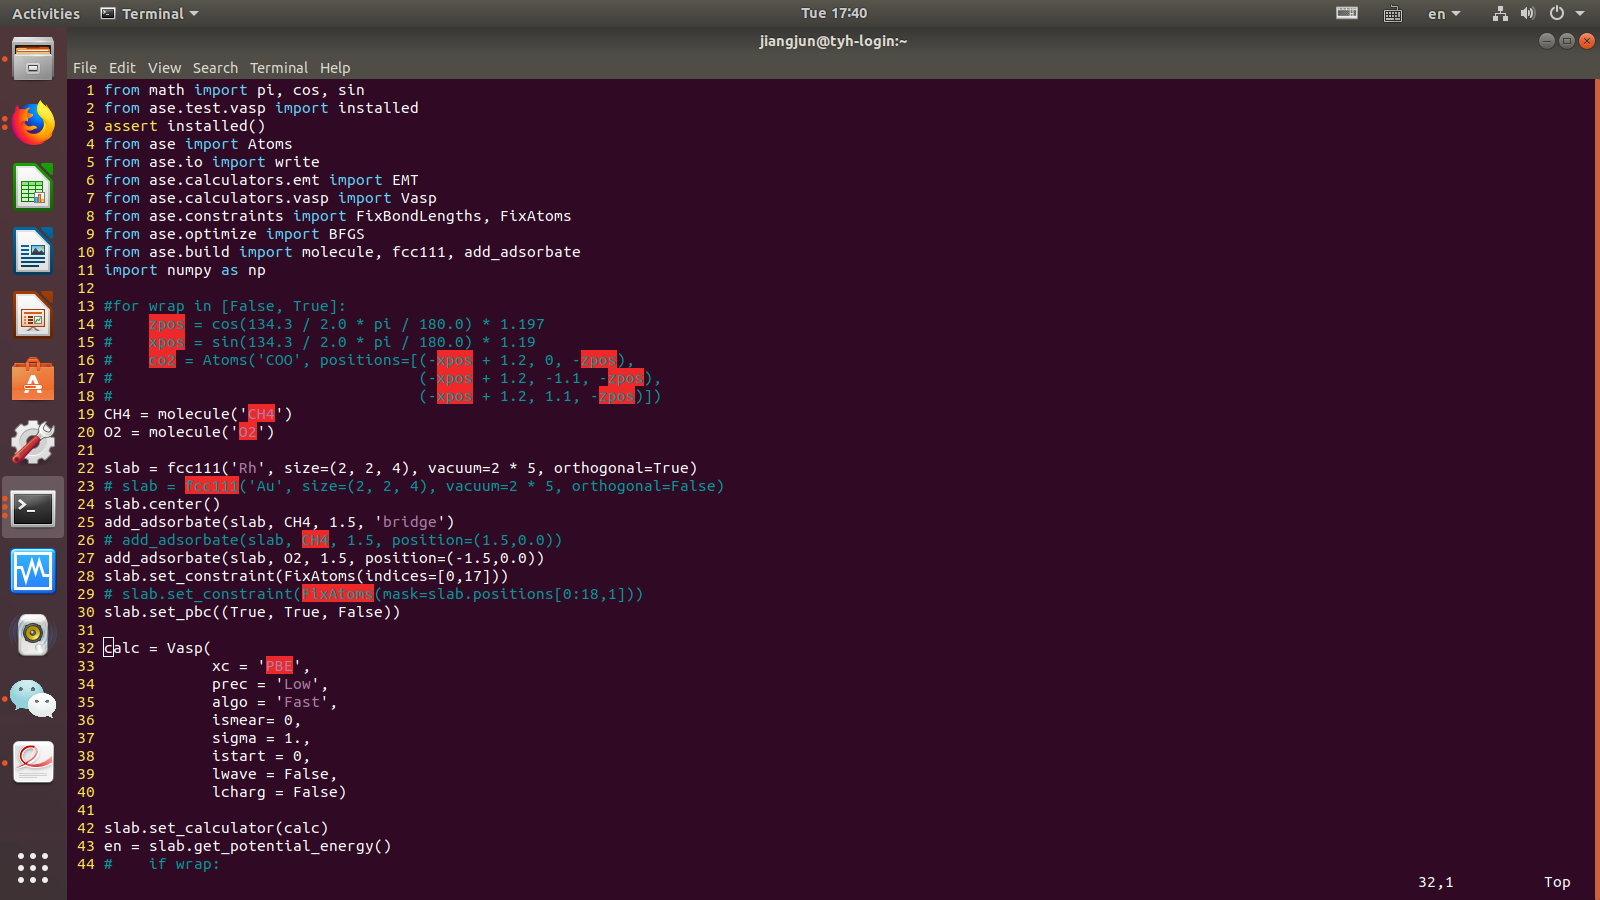
\includegraphics[height=3.1in,width=2.5in,viewport=75 0 725 820,clip]{Figures/ASE_app.png}
%%\caption{\fontsize{7.2pt}{4.2pt}\selectfont{\textrm{The integrated calculator in ASE (Atomic Simulation Environment).}}}%
%\label{ASE_app}
%\end{figure} 
%}

%\frame
%{
%	\frametitle{\textrm{计算平台的结果展示:~基于\textrm{MP}}}
%\begin{figure}[h!]
%\centering
%\vspace*{-0.2in}
%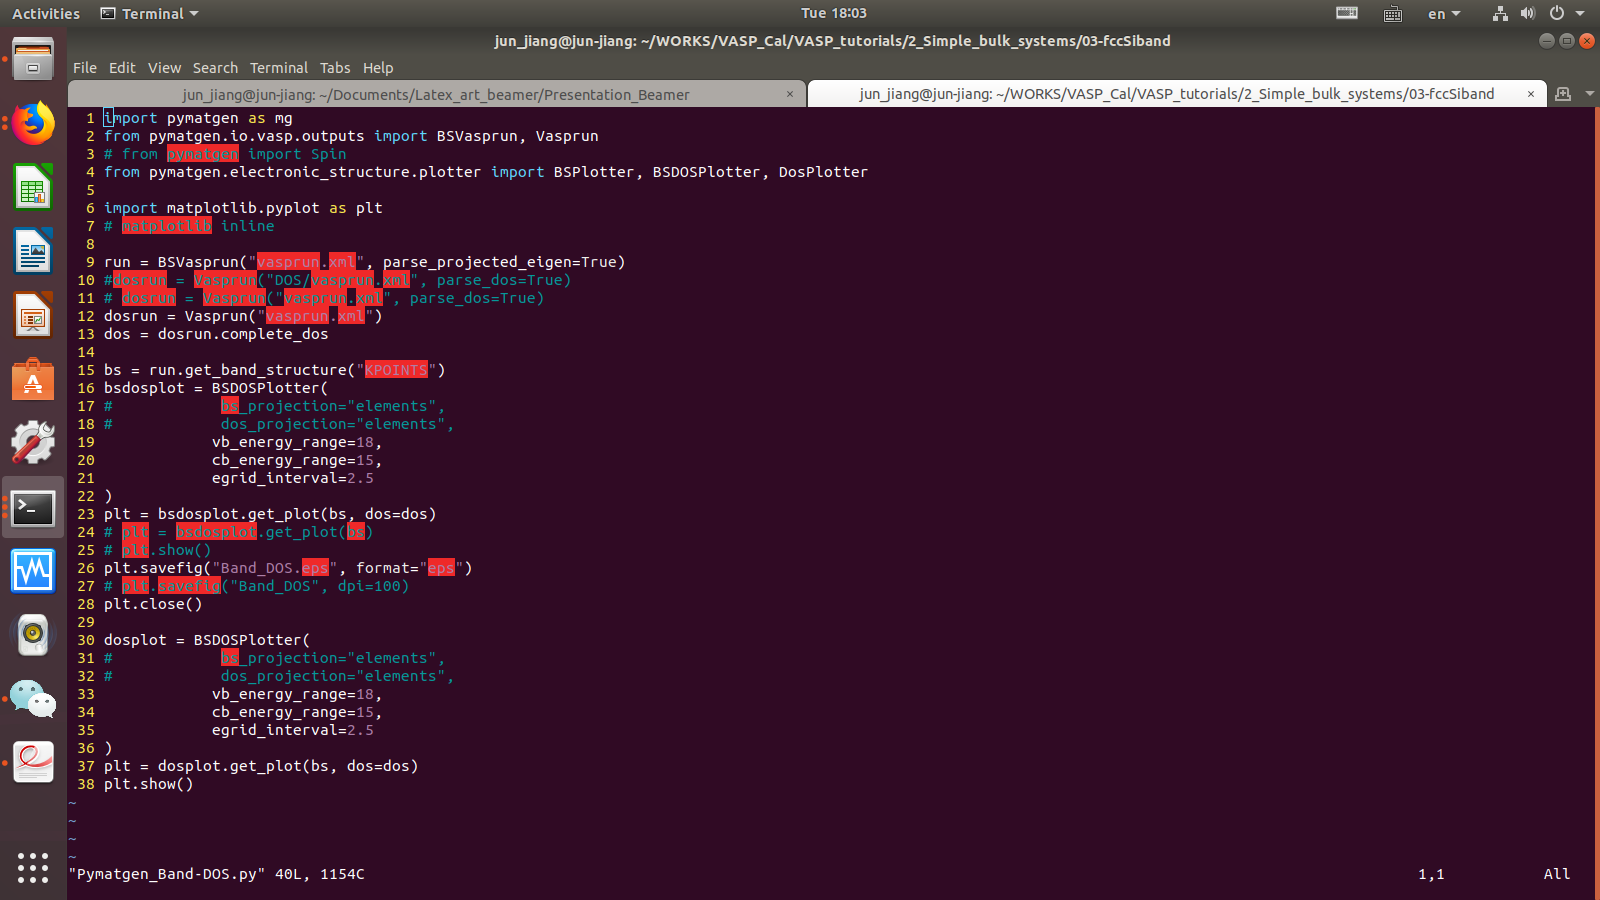
\includegraphics[height=3.1in,width=3.6in,viewport=73 80 880 790,clip]{Figures/Pymatgen_app.png}
%%\caption{\fontsize{7.2pt}{4.2pt}\selectfont{\textrm{The integrated calculator in ASE (Atomic Simulation Environment).}}}%
%\label{Pymatgen_app}
%\end{figure} 
%}
%
\frame
{
	\frametitle{调用\textrm{MP}与\textrm{ASE}封装模块}
\begin{figure}[h!]
\centering
\vspace*{-0.2in}
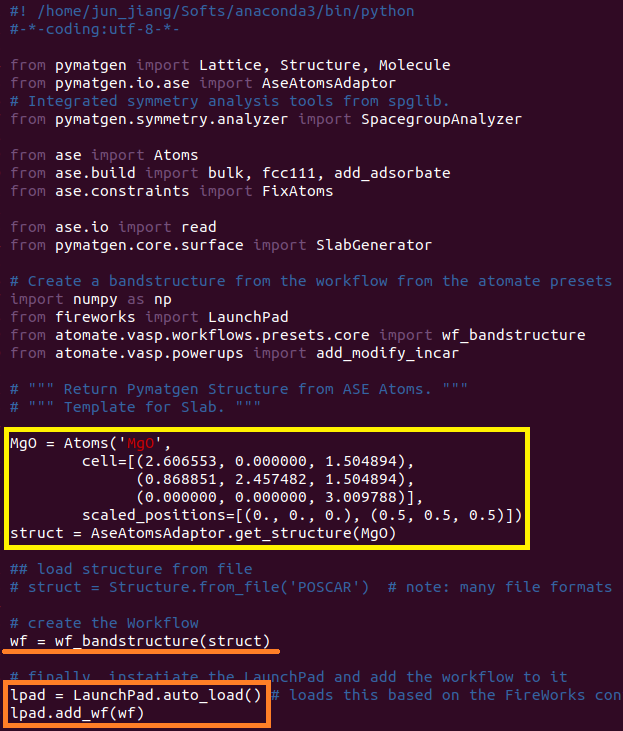
\includegraphics[height=3.0in,width=3.5in,viewport=0 0 600 550,clip]{Figures/Atomate-ASE_MgO.png}
%\caption{\fontsize{7.2pt}{4.2pt}\selectfont{\textrm{The integrated calculator in ASE (Atomic Simulation Environment).}}}%
\label{Atomate-ASE_app}
\end{figure} 
}

\frame
{
	\frametitle{应用示例:~\textrm{MgO:~DOS and Band}}
\begin{figure}[h!]
\centering
\vspace*{-0.2in}
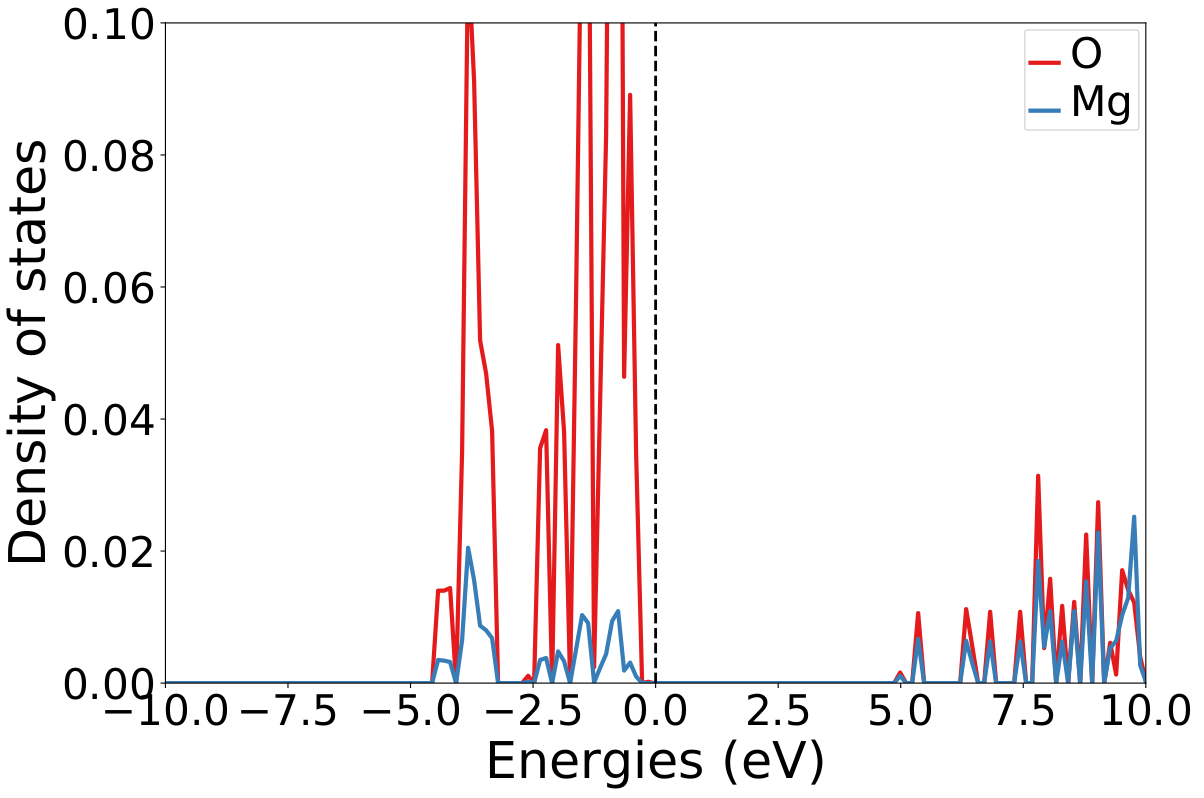
\includegraphics[height=1.5in,width=2.3in,viewport=0 0 900 600,clip]{Figures/Atomate_MgO-DOS.png}
\vskip 1pt
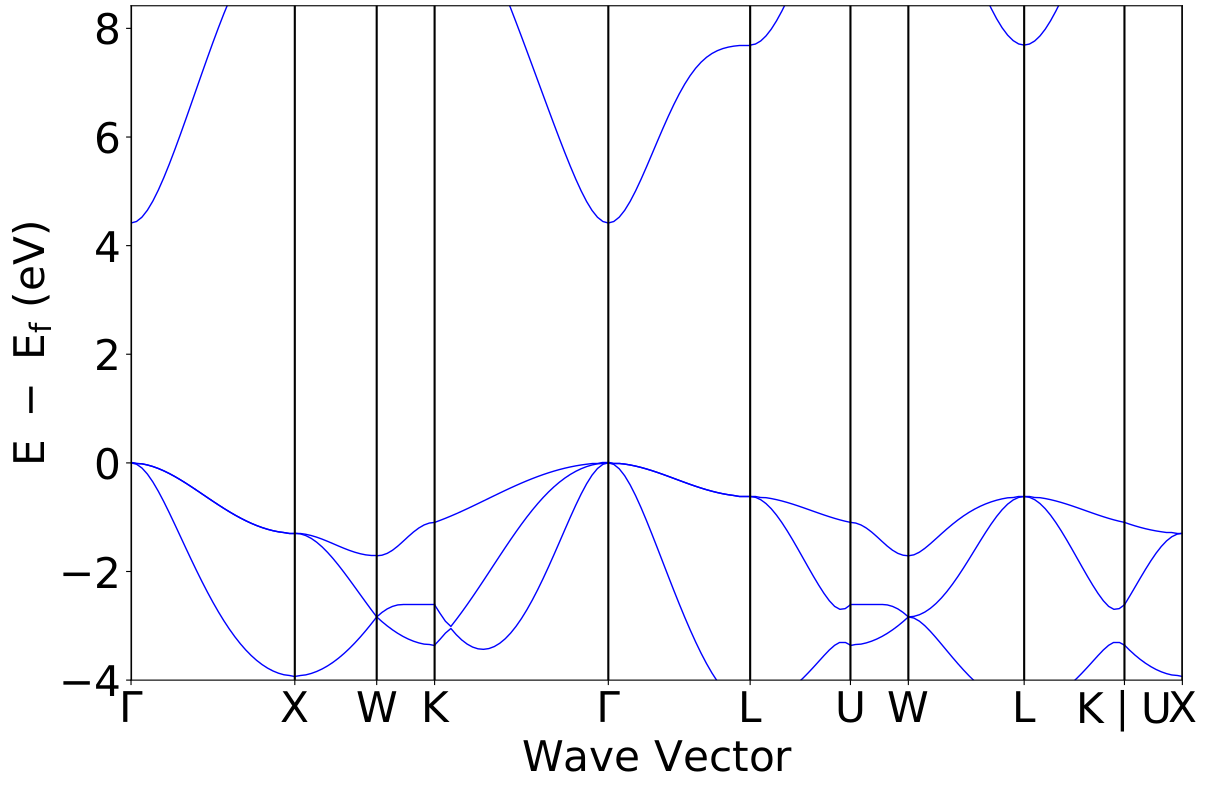
\includegraphics[height=1.5in,width=2.3in,viewport=0 0 900 600,clip]{Figures/Atomate_MgO-Band.png}
%\caption{\fontsize{7.2pt}{4.2pt}\selectfont{\textrm{The integrated calculator in Atomate-ASE.}}}%
\label{Atomate_MgO-DOS}
\end{figure} 
}

\section{\rm{VASP~}软件中的\rm{PAW~}方法}
\frame
{
%	\frametitle{\textrm{PAW}原子数据集}
	\frametitle{\textrm{PAW}方法的基本思想}
\begin{figure}[h!]
\centering
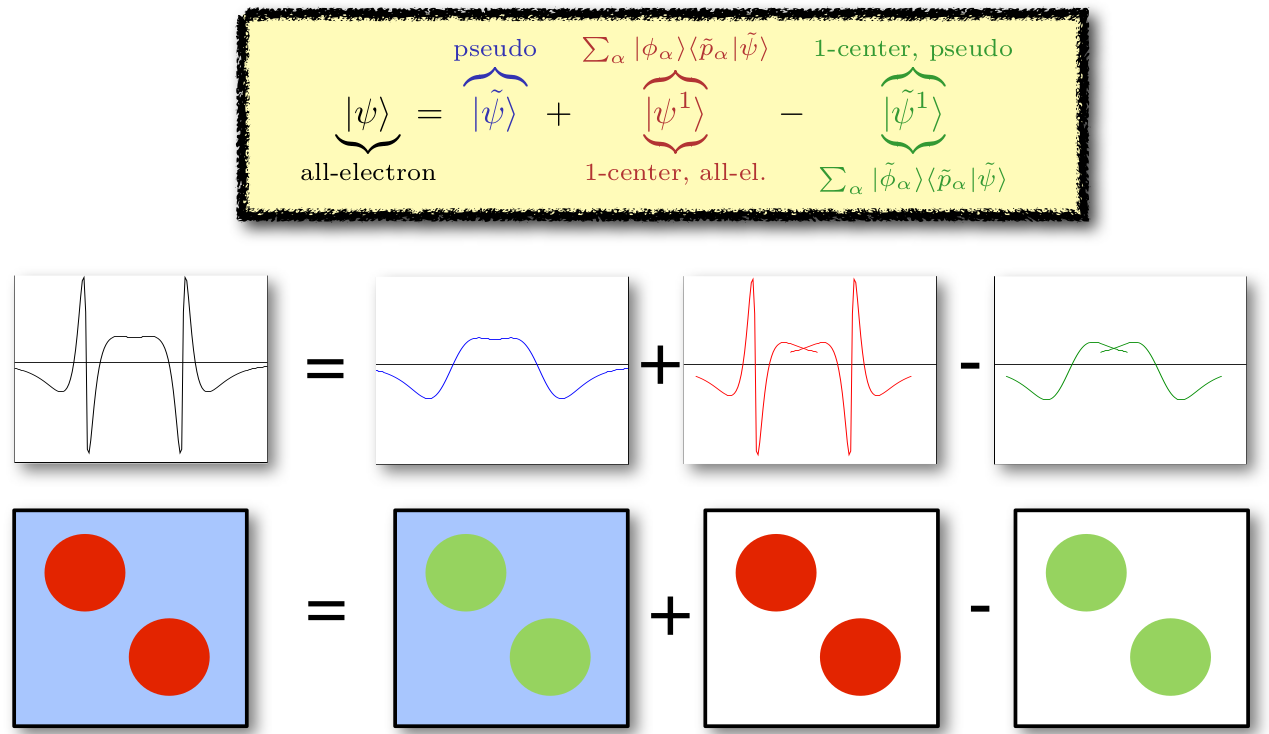
\includegraphics[height=2.3in,width=4.0in,viewport=0 0 1280 745,clip]{Figures/PAW-baseset.png}
\caption{\tiny \textrm{The Augmentation of PAW.}}%(与文献\cite{EPJB33-47_2003}图1对比)
\label{PAW_baseset}
\end{figure}
}

\frame
{
	\frametitle{\textrm{VASP}中的电荷密度的分解}
	\textrm{VASP}的开发者\textrm{G. Kresse}等明确了\textrm{PAW}方法与\textrm{USPP}方法的内在联系\upcite{PRB59-1758_1999}:
\begin{itemize}
	\item 芯层电荷与核电荷构成离子实电荷:$n_{Zc}=n_Z+n_c$
	\item 赝离子实电荷的构造$$\int_{\Omega_c}n_{Zc}(\vec r)\mathrm{d}^3\vec r=\int_{\Omega_c}\tilde n_{Zc}(\vec r)\mathrm{d}^3\vec r$$
\end{itemize}
在此基础上,\textrm{Bl\"ochl}方案中的电荷可以分解为:
\begin{displaymath}
	\begin{aligned}
		n_T=n+n_{Zc}\equiv&\underbrace{(\tilde n+\hat n+\tilde n_{Zc})}\\
				 		&\quad\qquad\tilde n_T\\
				  &+\underbrace{(n^1+\hat n+n_{Zc})}-\underbrace{(\tilde n^1+\hat n+\tilde n_{Zc})}\\
				                  &\quad\qquad n_T^1\qquad\qquad\qquad\tilde n_T^1
	\end{aligned}
\end{displaymath}
\textcolor{red}{注意}:\textrm{G. Kresse}方案中补偿电荷$\hat n$局域在每个缀加球内。
}

\frame
{
	\frametitle{总能量表达式}
	根据总能量表达式$$E=\tilde E+E^1-\tilde E^1$$其中
	\begin{displaymath}
		\begin{aligned}
			\tilde E=&\sum_nf_n\langle\tilde\Psi_n|-\frac12\nabla^2|\tilde\Psi_n\rangle+E_{\mathrm{XC}}[\tilde n+\hat n+\tilde n_c]+E_H[\tilde n+\hat n]\\
			&+\int v_H[\tilde n_{Zc}][\tilde n(\vec r)+\hat n(\vec r)]\mathrm{d}\vec r+U(\vec R,Z_{\mathrm{ion}})\\
			\tilde E^1=&\sum_{(i,j)}\rho_{ij}\langle\tilde\phi_i|-\frac12\nabla^2|\tilde\phi_j\rangle+\overline{E_{\mathrm{XC}}[\tilde n^1+\hat n+\tilde n_c]}+\overline{E_H[\tilde n^1+\hat n]}\\
			&+\int_{\Omega_r}v_H[\tilde n_{Zc}][\tilde n^1(\vec r)+\hat n(\vec r)]\mathrm{d}\vec r
		\end{aligned}
	\end{displaymath}
}

\frame
{
	\frametitle{总能量表达式}
	\begin{displaymath}
		\begin{aligned}
			E^1=&\sum_{(i,j)}\rho_{ij}\langle\phi_i|-\frac12\nabla^2|\phi_j\rangle+\overline{E_{\mathrm{XC}}[n^1+n_c]}+\overline{E_H[n^1]}\\
			&+\int_{\Omega_r}v_H[n_{Zc}]n^1(\vec r)\mathrm{d}\vec r
		\end{aligned}
	\end{displaymath}
	$v_H$是电荷密度$n$产生的静电势
	$$v_H[n](\vec r)=\int\dfrac{n(\vec r\,^{\prime})}{|\vec r-\vec r\,^{\prime}|}\mathrm{d}\vec r\,^{\prime}$$
	$E_H[n]$是对应的静电能
	$$E_H[n]=\dfrac12(n)(n)=\dfrac12\int\mathrm{d}\vec r\mathrm{d}\vec r\,^{\prime}\dfrac{n(\vec r)n(\vec r\,^{\prime})}{|\vec r-\vec r\,^{\prime}|}$$ 
	$U(\vec R,Z_{\mathrm{ion}})$\textcolor{blue}{由\textrm{Ewald}求和计算}
}

\frame
{
\frametitle{交换-相关能泛函的处理}
由于交换-相关能泛函是非线性的,\textrm{G. Kresse}方案中电荷密度分解为
\begin{displaymath}
	n_c+n=(\tilde n+\hat n+\tilde n_c)+(n^1+n_c)-(\tilde n^1+\hat n+\tilde n_c)
\end{displaymath}
原始的\textrm{Bl\"ochl}方案中电荷分解为
\begin{displaymath}
	n_c+n=(\tilde n)+(n^1+n_c)-(\tilde n^1)
\end{displaymath}
\textcolor{blue}{两种不同的电荷密度分解方案根源}:\\\textrm{G. Kresse}方案中赝离子实电荷$\tilde n_{Zc}$与\textrm{Bl\"ochl}方案中$\tilde n_c$的约束条件不同!
\begin{displaymath}
	E_{\mathrm{XC}}[\tilde n+\hat n+\tilde n_c]+\overline{E_{\mathrm{XC}}[n^1+n_c]}-\overline{E_{\mathrm{XC}}[\tilde n^1+\hat n+\tilde n_c]}
\end{displaymath}
}

\frame
{
	\frametitle{计算流程}
\begin{figure}[h!]
	\vspace{-0.2in}
\centering
%\includegraphics[height=2.7in,width=4.0in,viewport=0 0 1300 960,clip]{Figures/VASP_procedure-full.png}
%\includegraphics[height=2.1in,width=1.6in,viewport=0 0 480 630,clip]{Figures/VASP_procedure.png}
%\includegraphics[height=2.1in,width=2.3in,viewport=0 0 740 600,clip]{Figures/Ab-initio-Ene.png}
\includegraphics[height=2.5in,width=1.8in,viewport=0 0 480 630,clip]{Figures/VASP_procedure.png}
\caption{\tiny \textrm{The Flow of calculation for the KS-ground states.}}%(与文献\cite{EPJB33-47_2003}图1对比)
\label{PAW_baiseset}
\end{figure} 
}

%\frame
%{
%	\frametitle{\textrm{PAW Augmentation}}
%\begin{figure}[h!]
%\centering
%\includegraphics[height=2.3in,width=4.0in,viewport=0 0 1100 745,clip]{Figures/PAW-projector.png}
%\caption{\tiny \textrm{The projector of PAW.}}%(与文献\cite{EPJB33-47_2003}图1对比)
%\label{PAW_projector}
%\end{figure}
%}
%\frame
%{
%	\frametitle{赝势-\textrm{PAW}方法}
%\begin{figure}[h!]
%\centering
%%\hspace*{-0.80in}
%\includegraphics[height=1.0in,width=4.1in,clip]{Figures/Pseudo-Potential.png}
%\caption{\tiny \textrm{The relation of Pseudo potential and PAW.}}%(与文献\cite{EPJB33-47_2003}图1对比)
%\label{Pseudo_Poential}
%\end{figure}
%}
%
\subsection{\rm{POTCAR}的重构}
\frame
{
	\frametitle{\textrm{VASP}计算的原子数据基础}
	\textrm{POTCAR}提供了\textrm{VASP}计算所需的原子数据,也是实现\textrm{PAW}方法的主要基础
	\begin{itemize}
		\item \textrm{POTCAR}是\textrm{VASP}实现材料精确计算的重要保证\\
			同样都应用\textrm{PAW}方法,\textcolor{blue}{公认\textrm{VASP}较\textrm{QE}、\textrm{ABINIT}等软件的计算精度要高}
		\item \textrm{POTCAR}数据生成依赖较多的可调参数\\
			包括能量参数$\varepsilon_l$、多种截断半径$r_c$、$r_{\mathrm{vloc}}$、$r_{\mathrm{shape}}$、$r_{\mathrm{core}}$
		\item \textcolor{red}{\textrm{POTCAR}数据生成代码是\textrm{VASP}中唯一没有公开的}
		\item 用\textrm{VASP}模拟极端条件下材料物性的能力,受到\textrm{POTCAR}数据的制约
	\end{itemize}
	%文献\cite{PRB59-1758_1999}介绍了\textrm{POTCAR}的主要实现思想

当前研究主要尝试基于开源的\textrm{PAW}赝势生成软件(\textrm{atomPAW}),开发能生成\textrm{POTCAR}原子数据的功能
}

\frame
{
	\frametitle{\textrm{PAW}原子数据集:~\textrm{wave~function}}
	平滑赝原子分波函数
	\begin{displaymath}
		\tilde\phi_{i=Lk}(\vec r)=Y_L(\widehat{\vec r-\vec R})\tilde\phi_{lk}(|\vec r-\vec R|)
	\end{displaymath}
	根据\textrm{RRKJ}赝势构造的思想,赝分波函数由球\textrm{Bessel}函数线性组合\upcite{JPCM6-8245_1994}
	\begin{displaymath}
		\tilde\phi_{lk}(r)=\left\{
		\begin{aligned}
			&\sum_{i=1}^2\alpha_ij_l(q_ir)\quad &r<r_c^l\\
			&\phi_{lk}(r)\quad&r>r_c^l
		\end{aligned}
		\right.
	\end{displaymath}
	调节系数$\alpha_i$和$q_i$赝分波函数$\phi_{lk}(r)$在截断半径$r_c^l$处两阶连续可微
%	投影子波函数$\tilde p_i$由\textrm{Gram-Schmidt}正交条件$\langle\tilde p_i|\tilde\phi_j\rangle=\delta_{ij}$确定
}

\frame
{
	\frametitle{\textrm{PAW}原子数据集:~\textrm{wave~function}}
\begin{figure}[h!]
\centering
\vskip -0.5in
\includegraphics[width=1.5in,height=2.7in,viewport=0 0 350 550, angle=-90, clip]{Figures/WAE_data.eps}
\vskip -0.2in
\includegraphics[height=2.7in,width=1.5in,viewport=0 0 350 550, angle=-90, clip]{Figures/WPS_data.eps}
\caption{\tiny \textrm{The partial wave function.}}%(与文献\cite{EPJB33-47_2003}图1对比)
\label{Wave_Function}
\end{figure}
}

\frame
{
	\frametitle{\textrm{PAW}原子数据集:~\textrm{core~density}}
	\textcolor{blue}{构造赝芯电荷密度$\tilde n_c$}:~在截断半径$r_{\mathrm{core}}$内的定义为
	$$\sum_{i=1,2}B_i\dfrac{\sin(q_ir)}r\quad r<r_{\mathrm{core}}$$
	调节系数$q_i$和$B_i$使得赝芯电荷密度$\tilde n_c(r)$在截断半径$r_{\mathrm{core}}$处的两阶导数连续
\begin{figure}[h!]
\vskip -0.5in
\centering
\hspace*{-0.1in}
\includegraphics[width=1.5in,height=2.35in,viewport=0 0 350 550, angle=-90, clip]{Figures/CORE_data.eps}
\hspace*{-0.7in}
\includegraphics[height=2.35in,width=1.5in,viewport=0 0 350 550, angle=-90, clip]{Figures/PCORE_data.eps}
\caption{\tiny \textrm{The core density.}}%(与文献\cite{EPJB33-47_2003}图1对比)
\label{core_density_Function}
\end{figure}
}

\frame
{
	\frametitle{\textrm{PAW}原子数据集:~$\mathrm{v}_{e\!f\!f}(r)$与$\tilde{\mathrm{v}}_{e\!f\!f}(r)$}
	\textcolor{blue}{原子局域有效势$\mathrm{v}_{e\!f\!f}^a$}
\begin{figure}[h!]
\vskip -0.1in
\centering
\includegraphics[width=1.3in,height=2.4in,viewport=0 0 700 1200, angle=-90, clip]{Figures/POTAE.eps}
\caption{\tiny \textrm{The local atomic effective-Potential.}}%(与文献\cite{EPJB33-47_2003}图1对比)
\label{local_atomic_PP}
\end{figure}
	\textcolor{blue}{构造原子局域赝势$\tilde v_{e\!f\!f}^a$}%(\textcolor{red}{为防止\textrm{ghost band}})
	:%\\
	(在截断半径$r_{\mathrm{loc}}$内的定义)
	$$\tilde v_{e\!f\!f}^a=A\dfrac{\sin(q_{loc}r)}r\quad r<r_{\mathrm{loc}}$$
	其中$q_{loc}$和$A$要求局域赝势在截断半径$r_{\mathrm{loc}}$处连续到一阶导数
}

\frame
{
	\frametitle{\textrm{PAW}原子数据集:~$\mathrm{v}_H[\tilde n_{Zc}]$}
	局域离子赝势$v_H[\tilde n_{Zc}]$可由原子局域赝势去屏蔽得到
	$$v_H[\tilde n_{Zc}]=\tilde v_{e\!f\!f}^a-v_H[\tilde n_a^1+\hat n_a]-v_{\mathrm{XC}}[\tilde n_a^1+\hat n_a+\tilde n_c]$$
\begin{figure}[h!]
\vskip -0.5in
\centering
\hspace*{-0.1in}
\includegraphics[width=1.5in,height=2.35in,viewport=0 0 350 550, angle=-90, clip]{Figures/POTPS_data.eps}
\hspace*{-0.7in}
\includegraphics[height=2.35in,width=1.5in,viewport=0 0 350 550, angle=-90, clip]{Figures/POTPSC_data.eps}
\caption{\tiny \textrm{The pseudo-potential and local ionic pseudo-potential.}}%(与文献\cite{EPJB33-47_2003}图1对比)
\label{pseudo_potential}
\end{figure}
}

\frame
{
	\frametitle{\textrm{PAW}原子数据集:~倒空间$\tilde{\mathrm{v}}_{\mathrm{ion}}^a(G)$}和$\tilde n(G)$
	由势函数由实空间向倒空间的变换关系
	\begin{displaymath}
		\begin{aligned}
%			\textrm{v}(G)=&e^2\int\dfrac{\mathrm{d}^2r}{\mathrm r}\mathrm{e}^{\mathrm{i}\vec G\cdot\vec r}=2\pi e^2\int_0^{\infty}r\mathrm{d}r\int_{-1}^1\mathrm{d}(\cos\theta)\mathrm{e}^{\mathrm{i}Gr\cos\theta}\\
%			=&\dfrac{2\pi e^2}{\mathrm{i}G}\int_0^{\infty}\mathrm{d}r(\mathrm{e}^{\mathrm{i}Gr}-\mathrm{e}^{-\mathrm{i}Gr})=\dfrac{4\pi e^2}G\int_0^{\infty}\mathrm{d}r\sin(Gr)
			\textrm{v}(G)=&\int\mathrm{d}^3r v(r)\mathrm{e}^{\mathrm{i}\vec G\cdot\vec r}=2\pi \int_0^{\infty} v(r)\cdot r~r\mathrm{d}r\int_{-1}^1\mathrm{d}(\cos\theta)\mathrm{e}^{\mathrm{i}Gr\cos\theta}\\
			=&\dfrac{2\pi}{\mathrm{i}G}\int_0^{\infty}v(r)\cdot r~\mathrm{d}r(\mathrm{e}^{\mathrm{i}Gr}-\mathrm{e}^{-\mathrm{i}Gr})=\dfrac{4\pi}G\int_0^{\infty}\sin(Gr)v(r)\cdot r~\mathrm{d}r
		\end{aligned}
	\end{displaymath}
	可将$\mathrm{v}_H[\tilde n_{Zc}]$和$\tilde n(G)$变换为倒空间表示
\begin{figure}[h!]
\vskip -0.12in
\centering
\includegraphics[width=2.5in,height=1.4in,viewport=0 0 1200 630, clip]{Figures/PAW_Vloc_G.png}
\caption{\tiny \textrm{The pseudo-potential in reciprocal space.}}%(与文献\cite{EPJB33-47_2003}图1对比)
\label{pseudo_potential_G}
\end{figure}
}

%------------------------------------------------------------------------Reference----------------------------------------------------------------------------------------------
%\begin{thebibliography}{99}
%-----------------------------------------------------------------------------------------------------------------------------------------------------------------------%
%\frame
%{
%\frametitle{主要参考文献}
%{\small
%\bibitem{Singh_Book}\textrm{D. J. Singh. \textit{Plane Wave, PseudoPotential and the LAPW method} (Kluwer Academic, Boston,USA, 1994)}					%
%  \nocite{*}																				%
%}
%}
%\end{thebibliography}

\begin{thebibliography}{99}
\frame
{
\frametitle{主要参考文献}
\fontsize{6.5pt}{3.9pt}\selectfont{
	\bibitem{CMS146-319_2018}\textrm{X. Yang, Z. Wang, X. Zhao and H. Liu \textit{Comp. Mater. Sci.}, \textbf{146} (2018), 319}
	\bibitem{url_Matcloud}\textrm{\url{http://matcloud.cnic.cn}}
	\bibitem{CMS58-227_2012}\textrm{S. Curtarolo, W. Setyawan, S. Wang, J. Xue, K. Yang, R. H. Taylor, L. J. Nelson, G. L. Hart, S. Sanvito, M. Buongiorno-Nardelli, N. Mingo and O. Levy \textit{Comp. Mater. Sci.}, \textbf{58} (2012), 227}
	\bibitem{CMS97-209_2015}\textrm{S. P. Ong, S. Cholia, A. Jain, M. Brafman, D. Gunter, G. Ceder and K. A. Persson. \textit{Comp. Mater. Sci.}, \textbf{97} (2015), 209}
	\bibitem{url_QMIP}\textrm{\url{http://www.qmip.org/qmip.org/Welcome.html}}
	\bibitem{JPCL2-2241_2011}\textrm{J. Hachmann, R. Olivares-Amaya, S. Atahan-Evrenk, C. Amador-Bedolla, R. S. S$\acute{a}$nchez-Carrera, A. Gold-Parker, L. Vogt, A. M. Brockway and A. Aspuru-Guzik \textit{J. Phys. Chem. Lett.}, \textbf{2} (2011), 2241}
%	\bibitem{url_Mater_Genome}\textrm{\url{https://www.whitehouse.gov/sites/default/files/microsites/ostp/materials_genome_initiative-final.pdf}}
	\bibitem{CMS49-299_2010}\textrm{W. Setyawan and S. Curtarolo \textit{Comp. Mater. Sci.}, \textbf{49} (2010), 299}
	\bibitem{CMS50-2295_2011}\textrm{A. Jain, G. Hautier, C. J. Moore, S. P. Ong, C. C. Fischer, T. M. Kristin, K. A. Persson and G. Ceder \textit{Comp. Mater. Sci.}, \textbf{50} (2011), 2295}
	\bibitem{unpublished}\textrm{D. Gunter, S. Cholia, A. Jain, M. Kocher, K. Persson, L. Ramakrishnan, S. P. Ong and G. Ceder. \textit{Community Accessible Datastore of High-Throughput Calculations: Experiences from the Materials Project} (unpublished)}
}
\nocite*{}
}
\end{thebibliography}
%{\small
%-----------------------------------------------------------Beamer下不建议使用bib,因为涉及分页--------------------------------------------------------------------------%
%{\small
%\phantomsection\addcontentsline{toc}{section}{Bibliography}	 %直接调用\addcontentsline命令可能导致超链指向不准确,一般需要在之前调用一次\phantomsection命令加以修正	%
%\bibliography{Myref}																			%
%\bibliographystyle{mybib}																		%
%  \nocite{*}																				%
%}

%------------------------------------------------------------------------------------------------------------------------------------------------------------------------------%

%-------------------------------------------------------------------------Thanks------------------------------------------------------------------------------------------------
%\section{致谢}
%\frame
%{
%\frametitle{致$\quad$谢}
%\begin{itemize}
%    \setlength{\itemsep}{20pt}
%  \item 感谢本团队高兴誉、吴泉生、宋红州等各位老师参与的讨论
%  \item 感谢莫所长、宋主任以及软件中心各位老师和同事
%  \item 感谢王崇愚先生的帮助
%\end{itemize}
%}

\logo{}									%不显示logo
\frame
{
\vskip 60 pt
%\hskip 10pt \textcolor{blue}{\Huge 感谢答辩委员会各位老师\,\textrm{!}}\\
\vskip 35 pt
\hskip 60pt \textcolor{blue}{\Huge 谢谢大家\:!}
%\vskip 15 pt
%\hskip 40pt \textcolor{blue}{\Huge \textrm{for your attention\:!}}
}

%-------------------------------------------------------------------------------------------------------------------------------------------------------------------------------

\clearpage
%\end{CJK*}
\end{document}
